\documentclass[12pt]{article}
\usepackage{graphicx}
\usepackage[none]{hyphenat}
\usepackage[document]{ragged2e}
\usepackage[margin=1.0in]{geometry}
\usepackage{textcomp}

\usepackage{hyperref}
\hypersetup{
    colorlinks=true,
    linkcolor=blue,
    filecolor=magenta,      
    urlcolor=cyan,
    pdftitle={Quarter 1 Writeup},
    pdfpagemode=FullScreen,
}

\urlstyle{same}

\title{Predicting the Success of Baseball Pitchers \\ 
        \large Yilmaz Machine Learning 1 - 2022-2023}

\author{Wilson Chen and Bradley Cao}
\date{}
\begin{document}
\maketitle
\newpage{}
\tableofcontents
\newpage
\section{Introduction}
\subsection{Overview \& Rationale}
Major League Baseball (MLB) has become more and more statstics-driven over the years. Coaches use these statistics to evaluate player performance and make informed decisions about players, for example in draft reports. Contracts in MLB are often worth millions of dollars, so having statistics that measure player performance is extremely important. We wanted to see just how accurate predictions with these statistics are. For our project, we decided to look at a dataset on baseball pitchers. This dataset with 547 instances and 33 attributes contained information on different statistics recorded for pitchers. It came from the 2021 regular season, and only contained pitchers who had faced at least 100 batters. We wanted to see if we could use these statistics to predict whether or not a pitcher had a winning record. 

\subsection{Data Set Information}
We got our original dataset from \url{https://www.baseballsavant.mlb.com}. It contained 33 attributes: 
\begin{itemize}
    \item $\textbf{last\_name}$
    \item $\textbf{first\_name}$
    \item $\textbf{player\_id}$
    \item $\textbf{year}$
    \item $\textbf{p\_game}$
    \item $\textbf{p\_total\_hits}$
    \item $\textbf{p\_home\_run}$
    \item $\textbf{p\_strikeout}$
    \item $\textbf{p\_walk}$
    \item $\textbf{p\_k\_percent}$
    \item $\textbf{p\_bb\_percent}$
    \item $\textbf{batting\_avg}$
    \item $\textbf{slg\_percent}$
    \item $\textbf{on\_base\_percent}$
    \item $\textbf{on\_base\_plus\_slg}$
    \item $\textbf{p\_earned\_run}$
    \item $\textbf{p\_win}$
    \item $\textbf{p\_loss}$
    \item $\textbf{p\_era}$
    \item $\textbf{p\_rbi}$
    \item $\textbf{p\_called\_strike}$
    \item $\textbf{p\_unearned\_run}$
    \item $\textbf{exit\_velocity\_avg}$
    \item $\textbf{launch\_angle\_avg}$
    \item $\textbf{sweet\_spot\_percent}$
    \item $\textbf{barrel\_batted\_rate}$
    \item $\textbf{hard\_hit\_percent}$
    \item $\textbf{meatball\_percent}$
    \item $\textbf{pitch\_hand}$
    \item $\textbf{fastball\_avg\_speed}$
    \item $\textbf{n\_fastball\_formatted}$
    \item $\textbf{offspeed\_avg\_speed}$
    \item $\textbf{n\_offspeed\_formatted}$
\end{itemize}
These statistics were collected by MLB or MLBStatCast, a partner company that specializes in collecting data from MLB games.  

\section{Preprocessing}
\subsection{Missing and Redundant Values}
We first started by removing redundant values, such as OPS. The OPS attribute is just the sum of the On Base Percentage ($\textbf{OBP}$) and Slugging ($\textbf{SLG}$), so we can safely remove it without losing any information. Furthermore, there were missing values for the attributes Offspeed\% and Offspeed Average MPH. We decided to remove these attributes altogether, as these values are missing because not all pitchers have an offspeed pitch; filling this data with an average would not be representative, and removing these attributes helps with dimensionality reduction. We also removed all attributes that did not relate to pitcher\textquotesingle s performance ($\textbf{name}$, $\textbf{year}$, $\textbf{player}$ $\textbf{ID}$, etc.). We can safely remove these attributes since they provide zero information. 
\newpage{}
\subsection{Class Labels}
Since our data did not come with class labels, we had to create them ourselves. Using the $\textbf{p\_win}$ and $\textbf{p\_loss}$, we created our own column, titled $\textbf{winning}$ to keep track of whether or not the pitcher had a winning record. For pitchers that had an even record, with the same number of wins and losses, we classified them as having a winning record. We then removed the attributes $\textbf{p\_win}$ and $\textbf{p\_loss}$ because the information they give us is given by our new class variable. 

\subsection{Dimensionality Reduction}

\subsubsection{Self Selection}
The first method we used was self selection. We picked 6 attributes that we believed, with our knowledge of baseball, would be the best indicators of a pitcher having a winning record. 

\newpage
\subsubsection{WrapperSubsetEval}
$\textbf{WrapperSubsetEval}$ is the first of the WEKA built-in attribute selection methods. It uses a learning scheme to evaluate attribute sets, and uses cross validation to estimate its accuracy for each set. 
\begin{figure}[h!]
    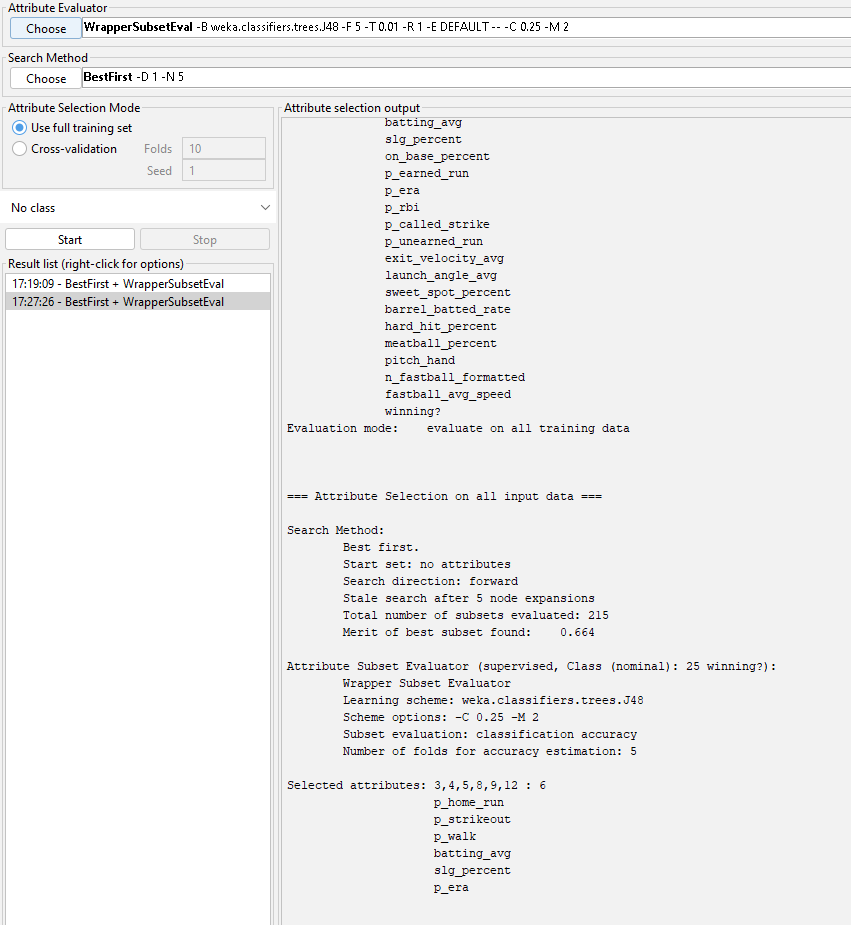
\includegraphics[scale=0.5]{./images/WrapperSubsetEval/WrapperSubsetEval.png}
    \centering
    \caption{WEKA screenshot showing the results of WrapperSubsetEval}
    \label{fig:Wrapper}
\end{figure}

\newpage
\subsubsection{InfoGainAttributeEval}
$\textbf{InfoGainAttributeEval}$ is the second WEKA built-in attribute selection method. It measures the information gain of each attribute relative to the class variable and gives us the ones with the most information gain, which are the most predictive of the class variable. 
\begin{figure}[h!]
    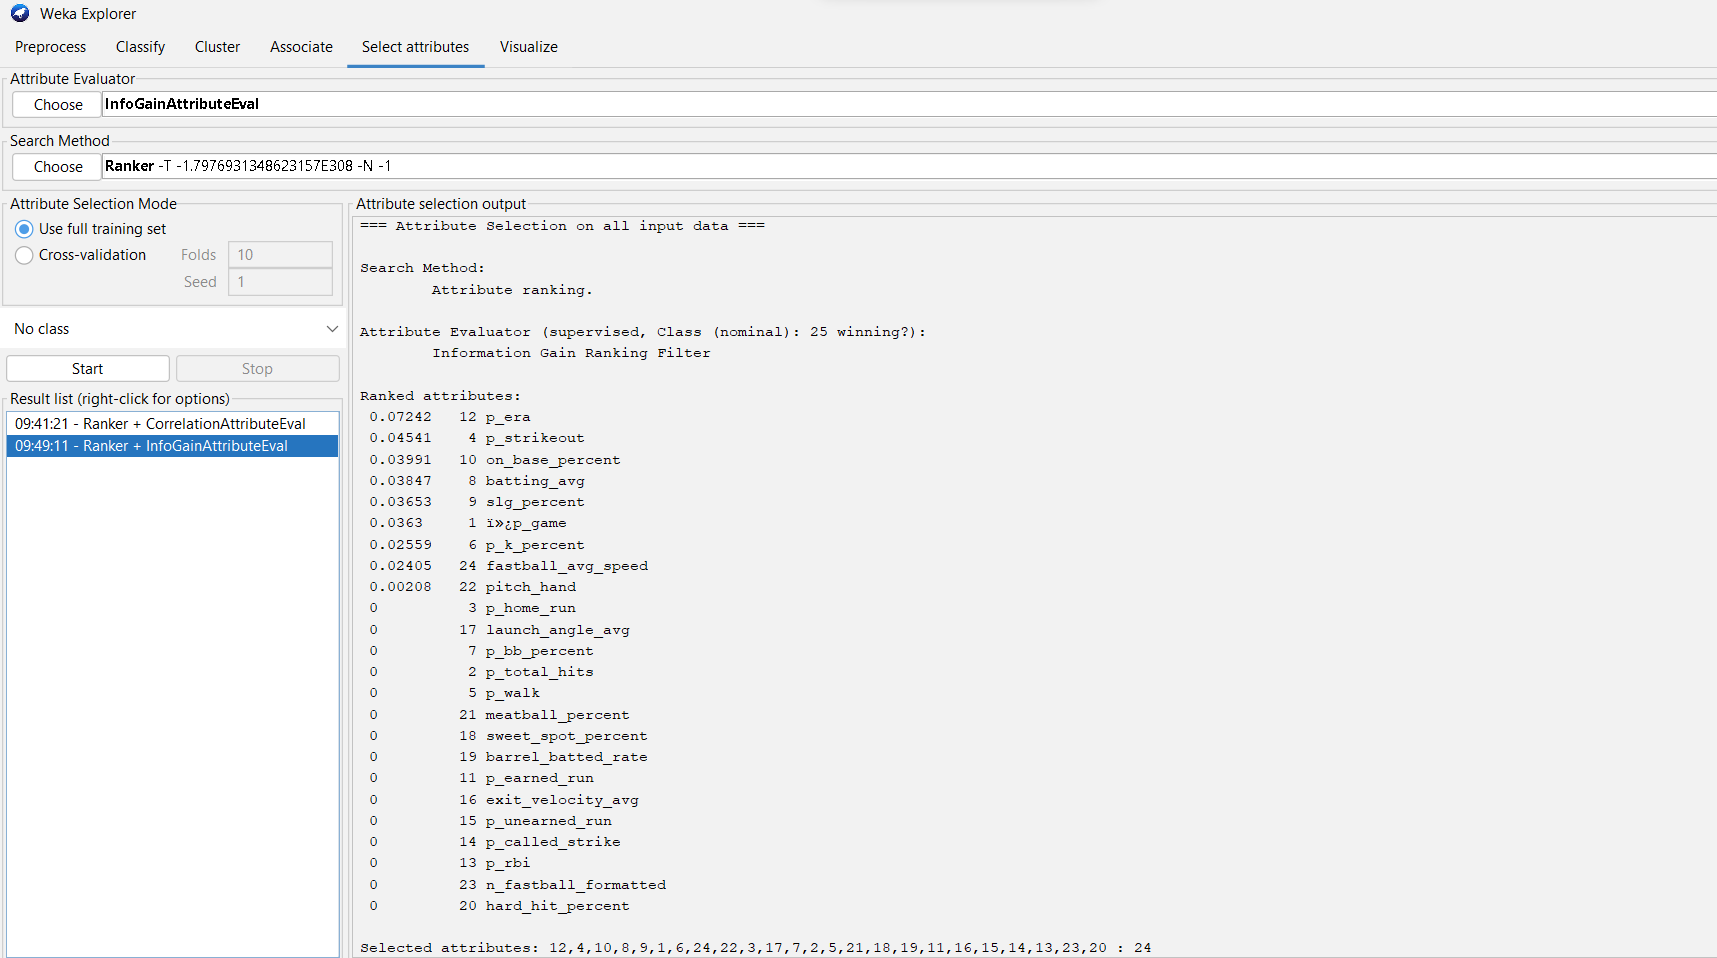
\includegraphics[scale=0.4]{./images/InfoGainAttributeEval/InfoGainAttributeEval.png}
    \centering
    \caption{WEKA screenshot showing the results of InfoGainAttributeEval}
    \label{fig:InfoGain}
\end{figure}

\newpage
\subsubsection{GainRatioAttributeEval}
$\textbf{GainRatioAttributeEval}$ is the third WEKA built-in attribute selection method. This method is similar to the previous, but instead measures the gain ratio for each attribute relative to the class variable. The gain ratio is the ratio of information gain to intrinsic information. 
\begin{figure}[h!]
    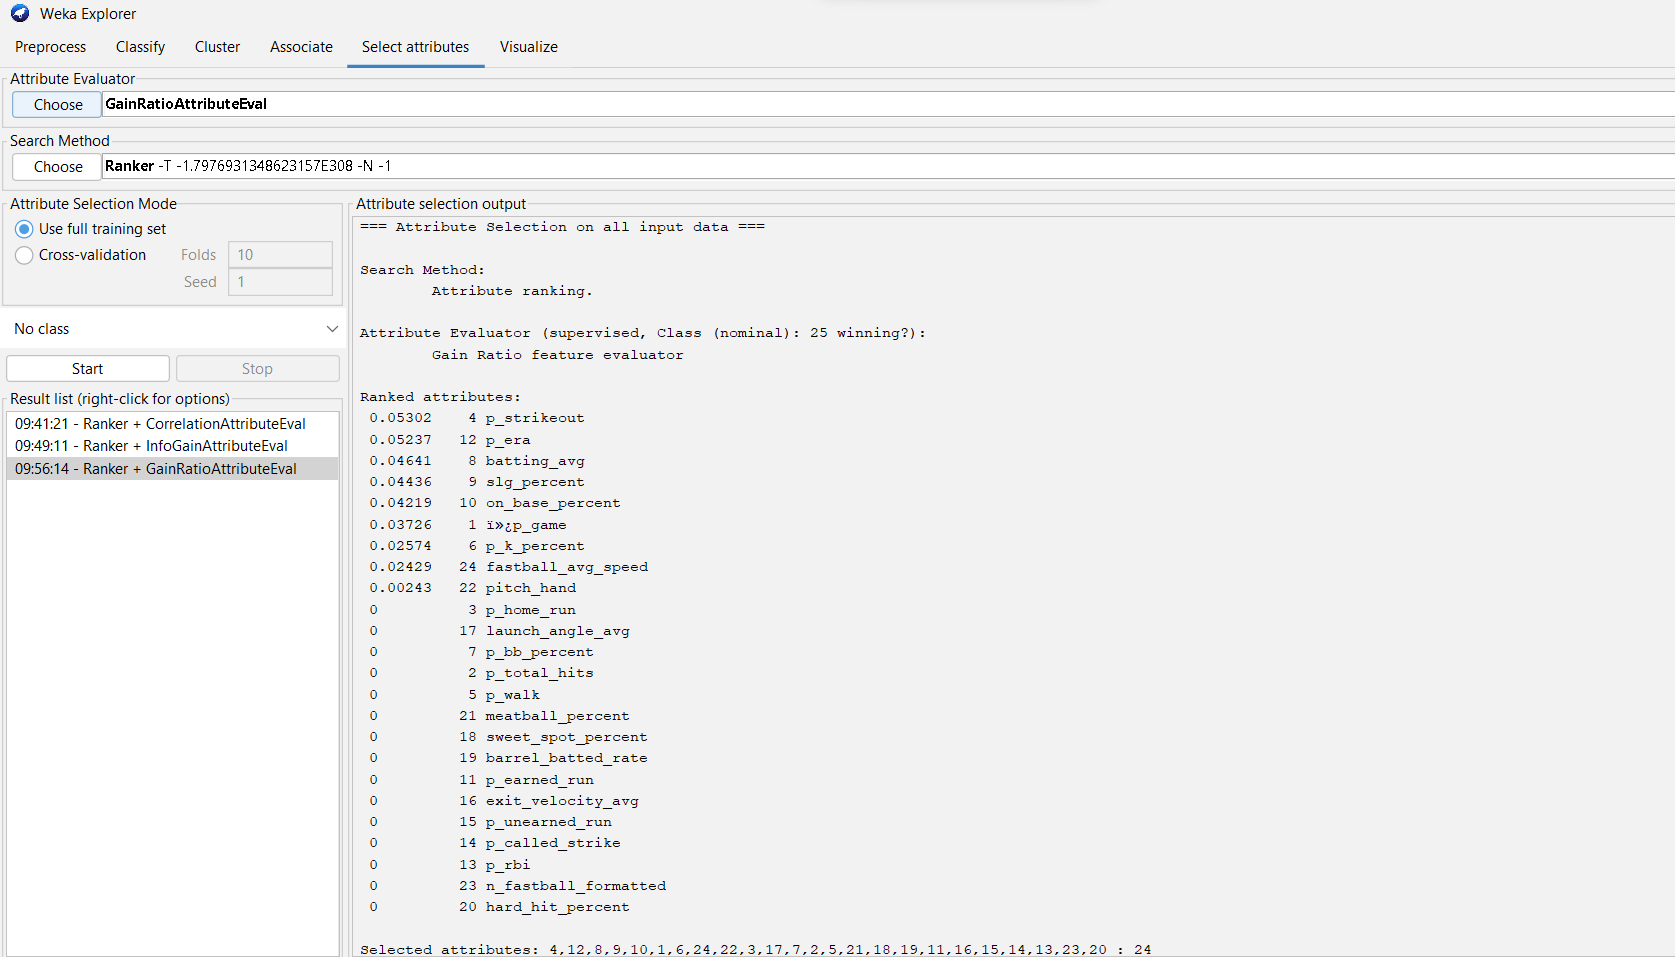
\includegraphics[scale=0.45]{./images/GainRatioAttributeEval/GainRatioAttributeEval.png}
    \centering
    \caption{WEKA screenshot showing the results of GainRatioAttributeEval}
    \label{fig:GainRatio}
\end{figure}

\newpage
\subsubsection{CorrelationAttributeEval}
$\textbf{CorrelationAttributeEval}$ is the final WEKA built-in attribute selection method we used. This method measures the Perason\textquotesingle s correlation between an attribute and the class variable. The Perason\textquotesingle s correlation measures the strength of a linear relationship between two varaibles, and can range from $-1$ to $1$. 
\begin{figure}[h!]
    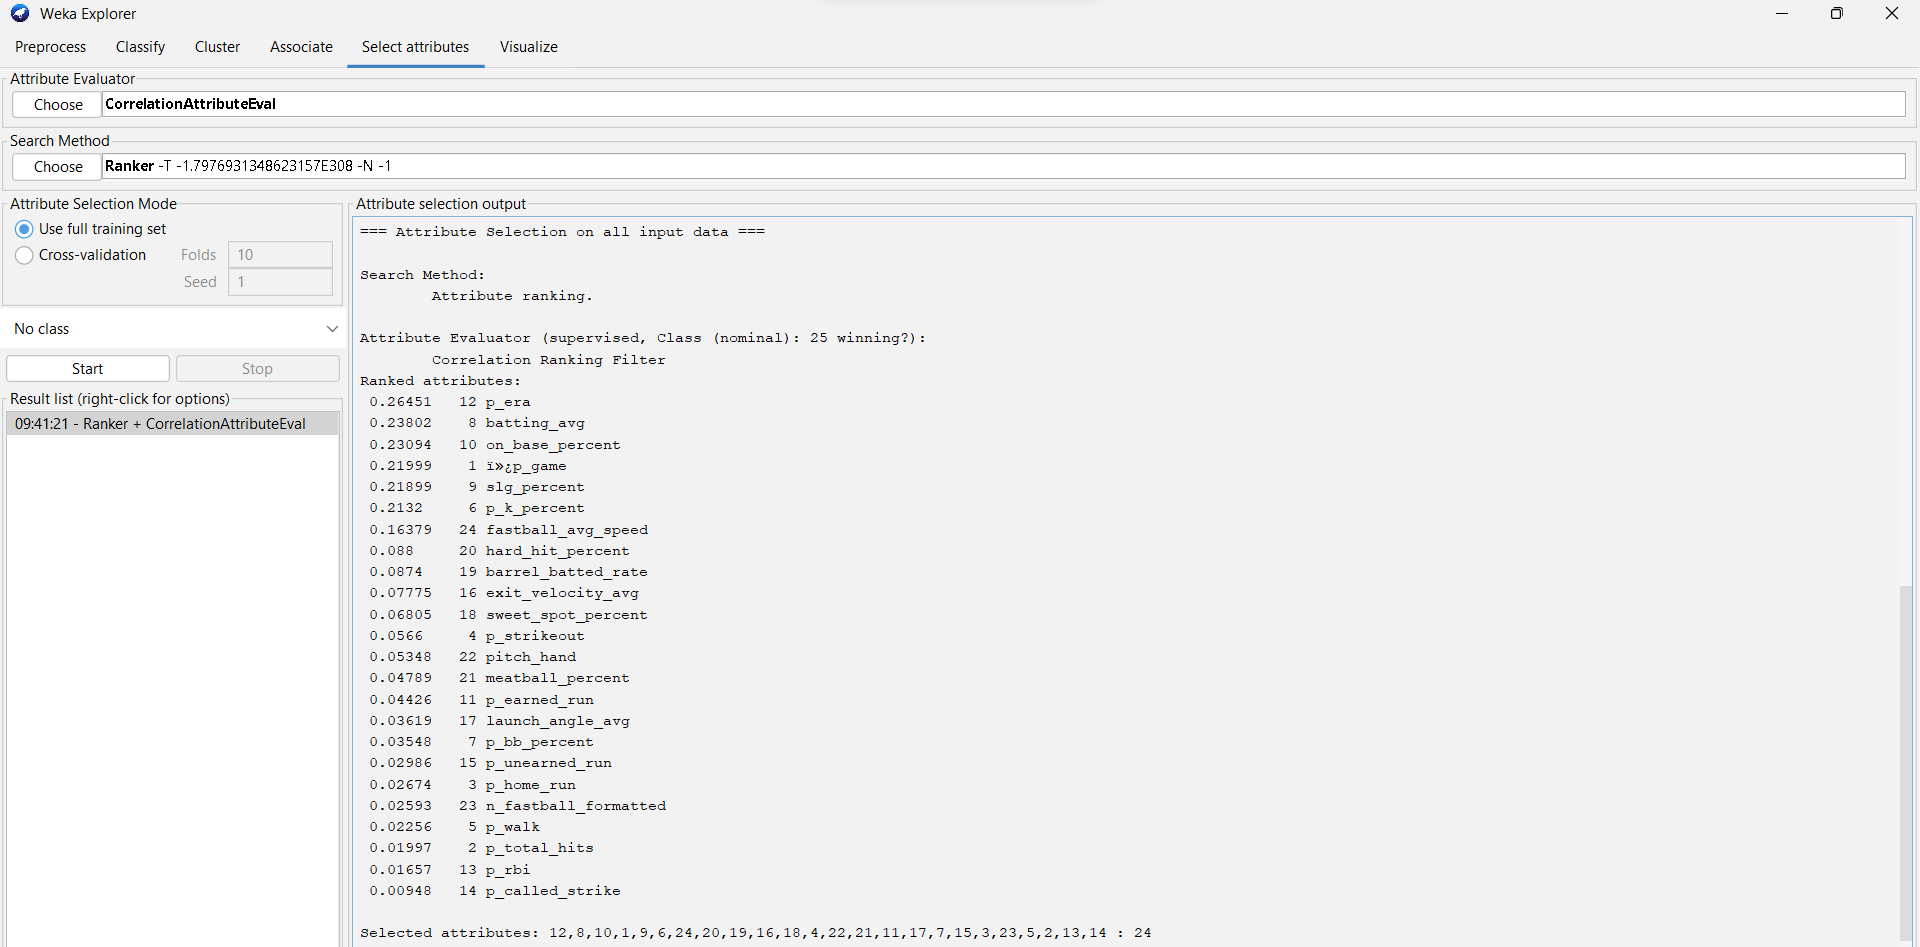
\includegraphics[scale=0.4]{./images/CorrelationAttributeEval/CorrelationAttributeEval.png}
    \centering
    \caption{WEKA screenshot showing the results of CorrelationAttributeEval}
    \label{fig:Correlation}
\end{figure}

\section{Splitting into Testing and Training}
For each one of these attribute selection methods, we removed all attributes except the ones selected and the class varaible. We then split the instances into a testing set and a training set using WEKA. For this, we used WEKA\textquotesingle s supervised filter $\textbf{Resample}$, which we configured to produce a random subset of the dataset without replacement. We ran it once, with the size of the output dataset to be 33\% of the whole to get the testing sets, then used the $\textbf{InvertSelection}$ feature to get the training sets. The training sets had $368$ instances, with $226$ classified as $\textbf{yes}$ and $142$ classified as $\textbf{no}$, while the testing sets had $179$ instances, with $110$ classified as $\textbf{yes}$ and $69$ classified as $\textbf{no}$.

\newpage
\subsection{SelfSelection}
\begin{figure}[h!]
    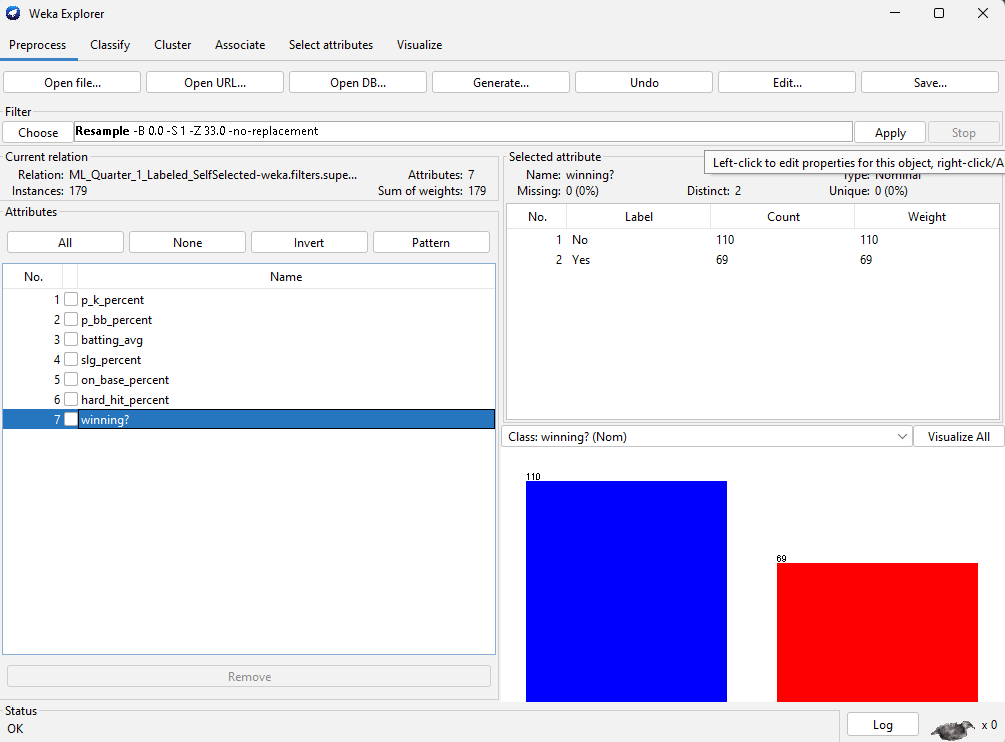
\includegraphics[scale=0.4]{./images/SelfSelected/TestSet.png}
\centering
    \caption{SelfSelection Test Set}
    \label{fig:SSTest}
\end{figure}
\begin{figure}[h!]
    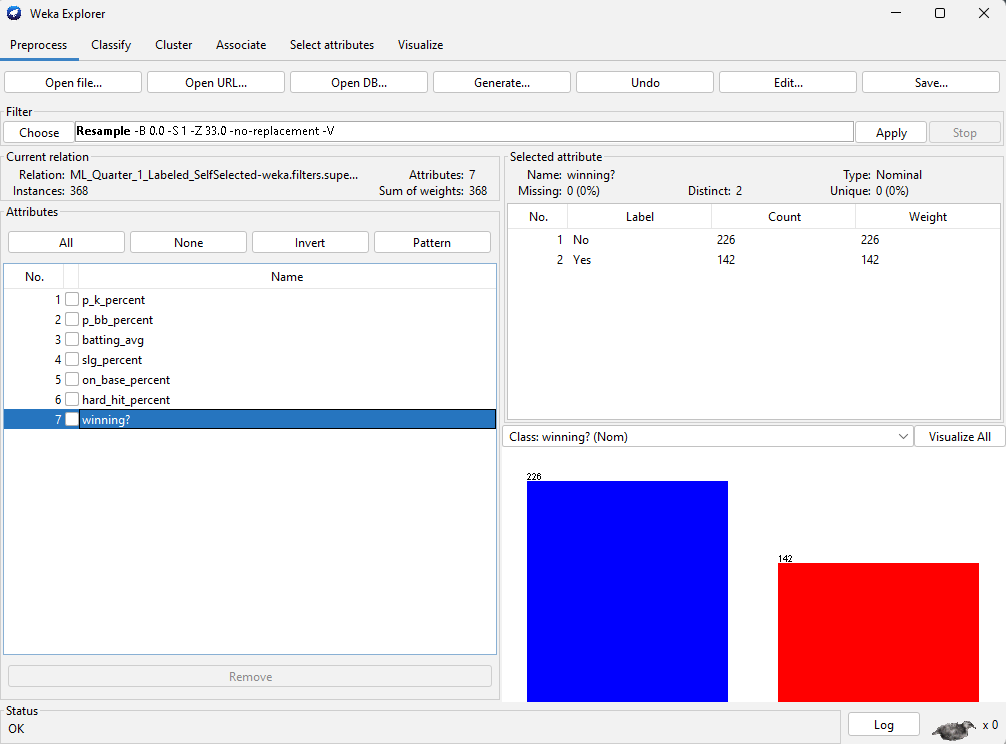
\includegraphics[scale=0.4]{./images/SelfSelected/TrainSet.png}
\centering
    \caption{SelfSelection Train Set}
    \label{fig:SSTrain}
\end{figure}

\newpage
\subsection{WrapperSubsetEval}
\begin{figure}[h!]
    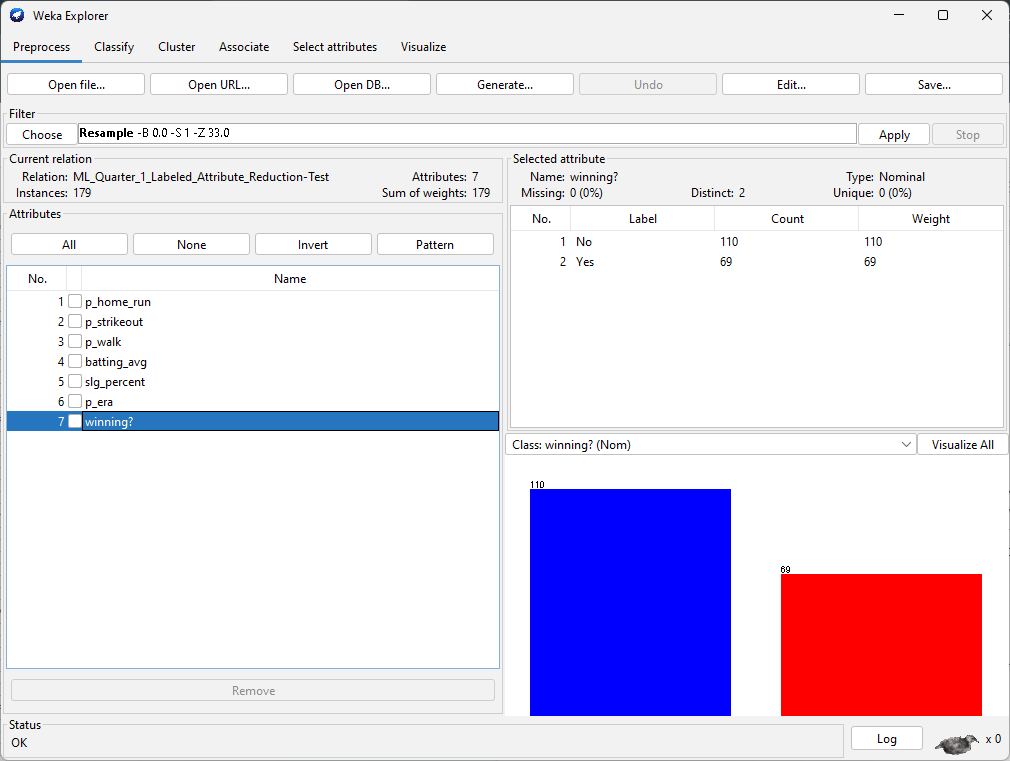
\includegraphics[scale=0.4]{./images/WrapperSubsetEval/TestSet.png}
\centering
    \caption{WrapperSubsetEval Test Set}
    \label{fig:WSETest}
\end{figure}
\begin{figure}[h!]
    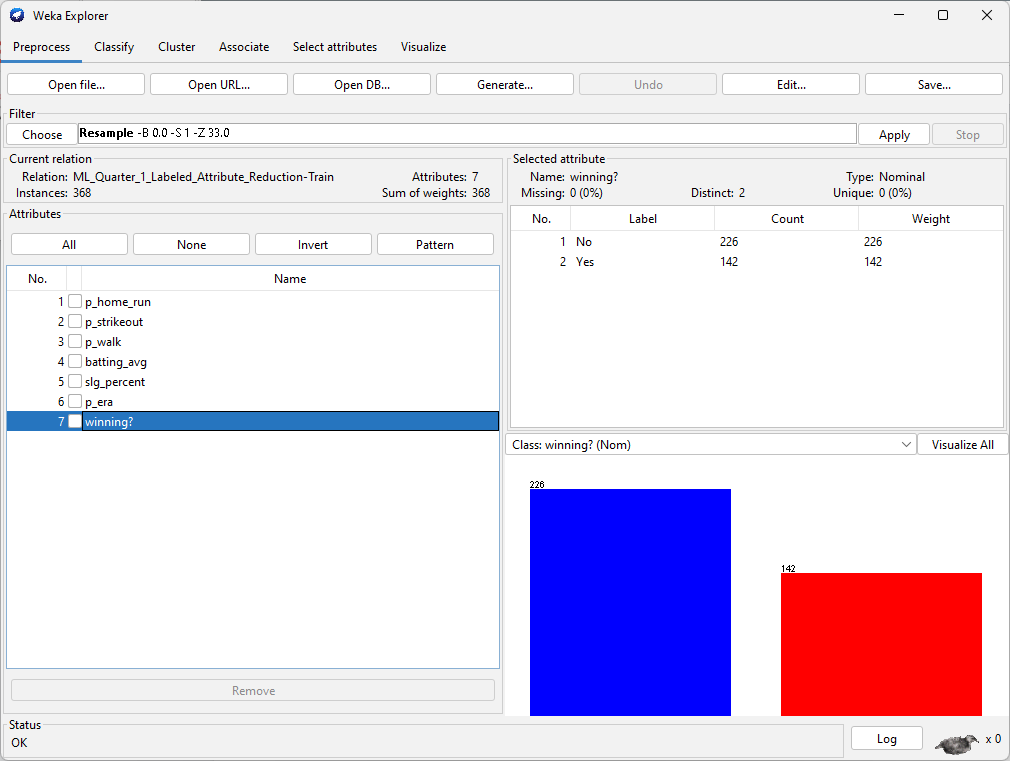
\includegraphics[scale=0.4]{./images/WrapperSubsetEval/TrainSet.png}
\centering
    \caption{WrapperSubsetEval Train Set}
    \label{fig:WSETrain}
\end{figure}

\newpage
\subsection{InfoGainAttributeEval}
\begin{figure}[h!]
    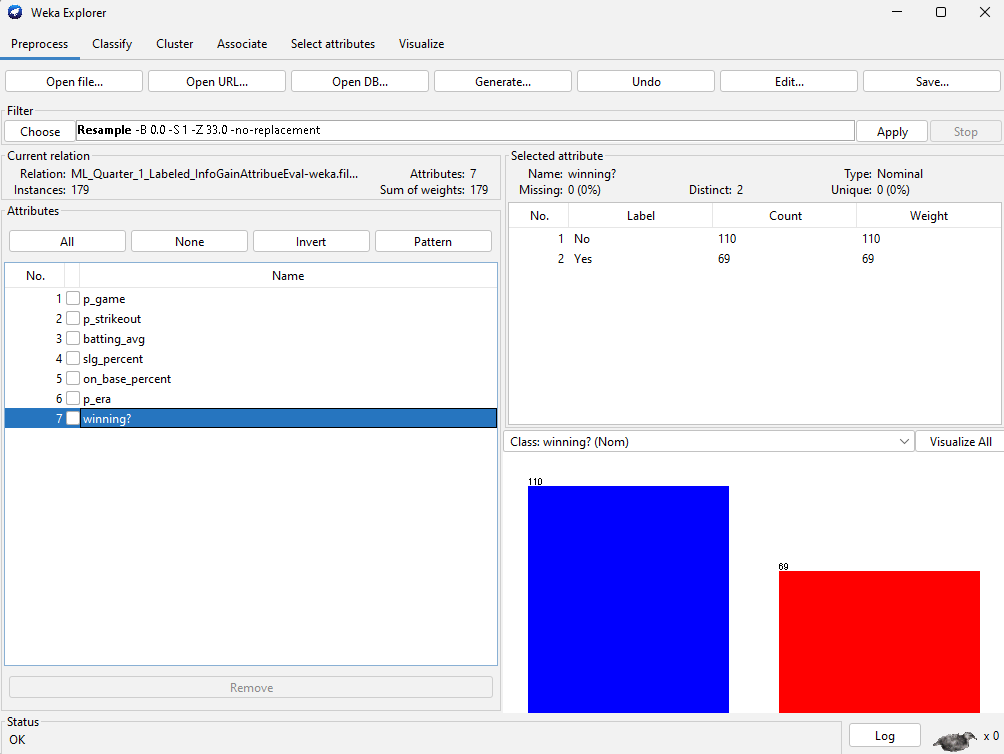
\includegraphics[scale=0.4]{./images/InfoGainAttributeEval/TestSet.png}
\centering
    \caption{InfoGainAttributeEval Test Set}
    \label{fig:IGAETest}
\end{figure}
\begin{figure}[h!]
    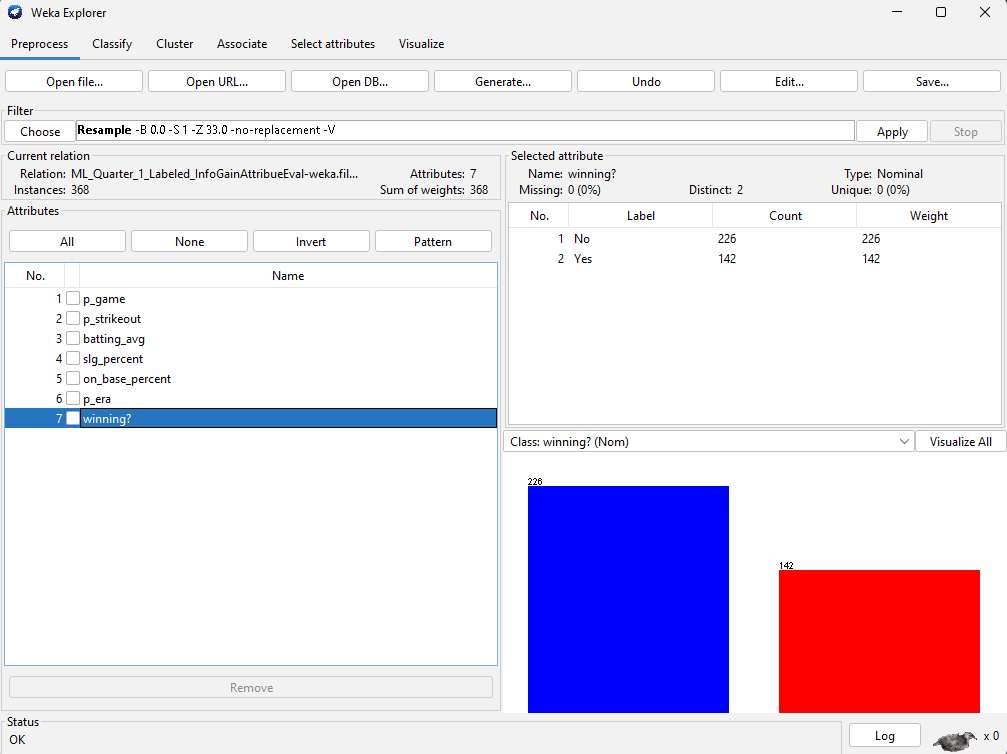
\includegraphics[scale=0.4]{./images/InfoGainAttributeEval/TrainSet.png}
\centering
    \caption{InfoGainAttributeEval Train Set}
    \label{fig:IGAETrain}
\end{figure}

\newpage
\subsection{GainRatioAttributeEval}
\begin{figure}[h!]
    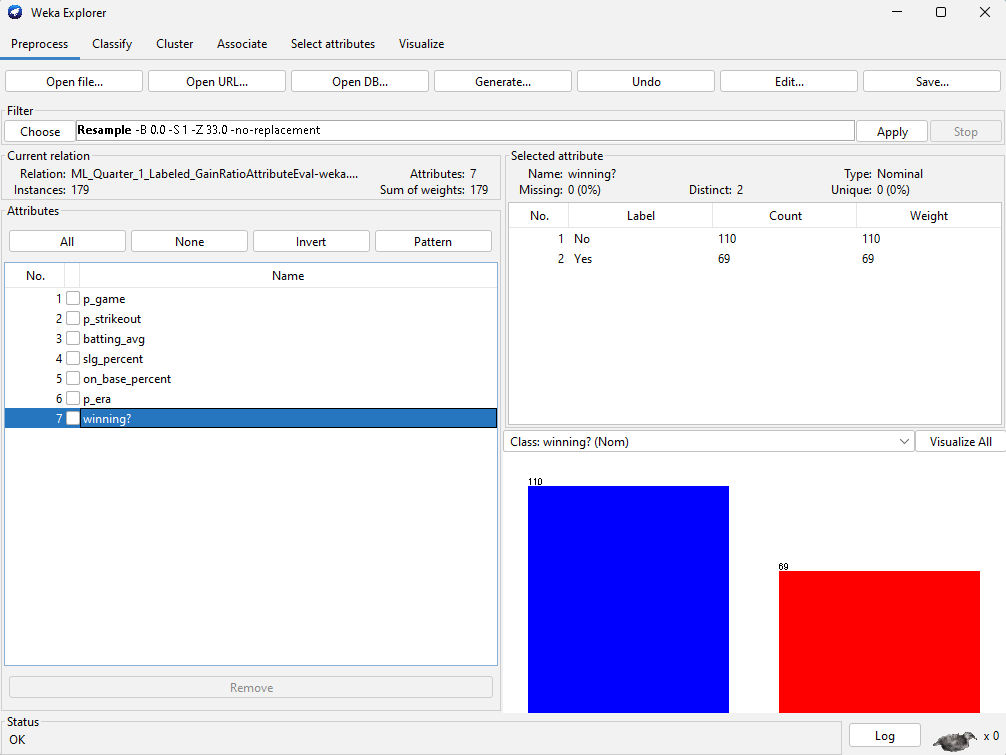
\includegraphics[scale=0.4]{./images/GainRatioAttributeEval/TestSet.png}
\centering
    \caption{GainRatioAttributeEval Test Set}
    \label{fig:GRAETest}
\end{figure}
\begin{figure}[h!]
   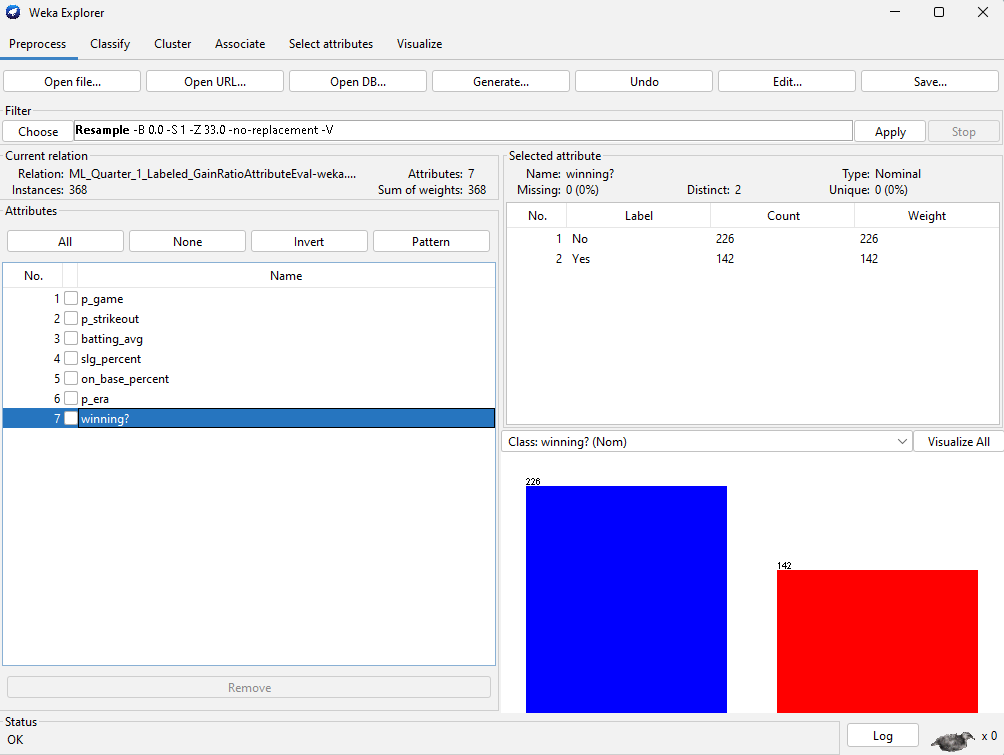
\includegraphics[scale=0.4]{./images/GainRatioAttributeEval/TrainSet.png}
\centering
    \caption{GainRatioAttributeEval Train Set}
    \label{fig:GRAETrain}
\end{figure}

\newpage
\subsection{CorrelationAttributeEval}
\begin{figure}[h!]
    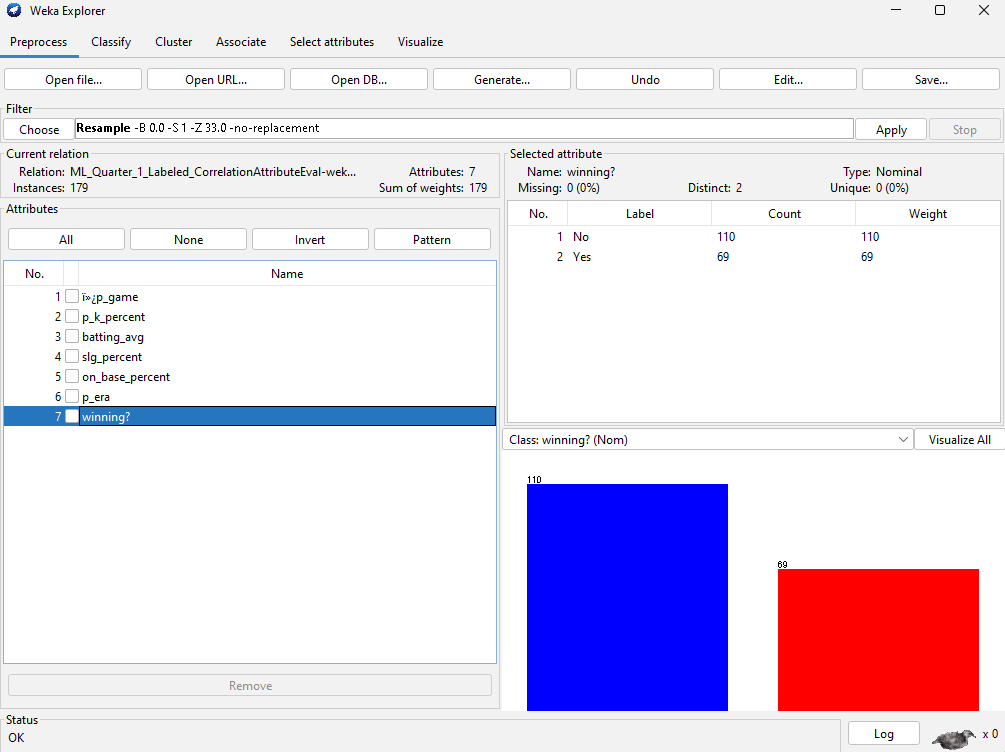
\includegraphics[scale=0.4]{./images/CorrelationAttributeEval/TestSet.png}
\centering
    \caption{CorrelationAttributeEval Test Set}
    \label{fig:CAETest}
\end{figure}
\begin{figure}[h!]
   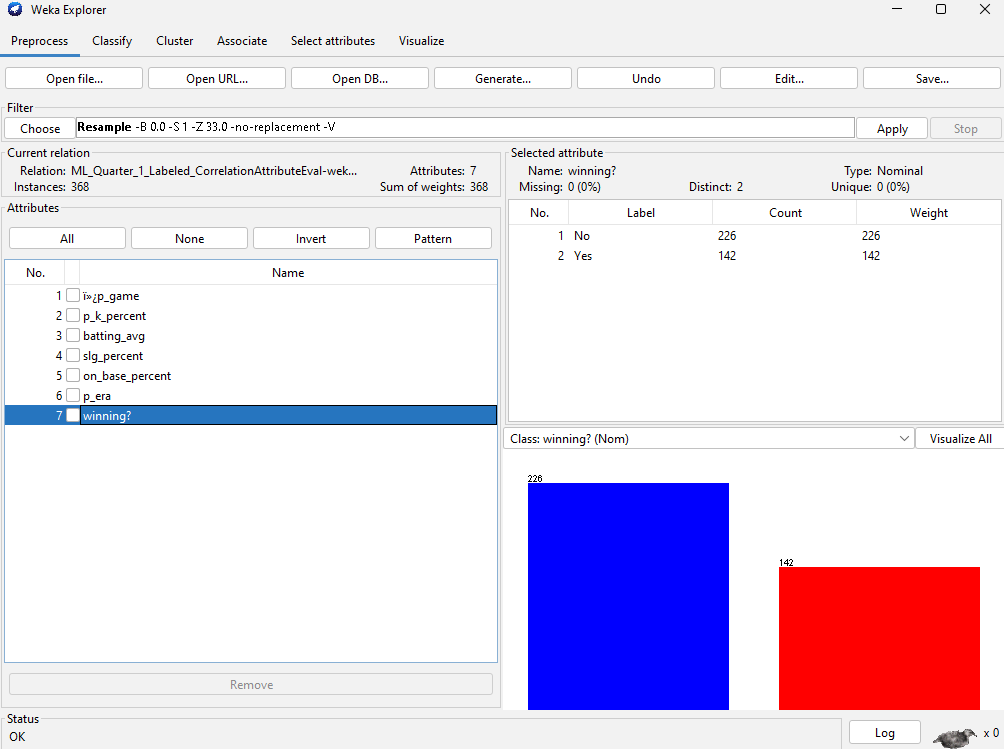
\includegraphics[scale=0.4]{./images/CorrelationAttributeEval/TrainSet.png}
\centering
    \caption{CorrelationAttributeEval Train Set}
    \label{fig:CAETrain}
\end{figure}

\newpage
\section{Classification}
For each method of attribute reduction, we ran $4$ classification methods using WEKA. These methods included: 
\begin{itemize}
    \item $\textbf{J48}$
    \item $\textbf{LogisticFunction}$
    \item $\textbf{NaiveBayes}$
    \item $\textbf{OneR}$
\end{itemize}
We compared each of these methods to determine which one worked the best for each attribute reduction method. They were trained using supplied training sets we created earlier. We then tested each classification method on each of the testing sets that we created, running $20$ classifications in total.

\subsection{Types of Classification Methods}
\subsubsection{J48}
$\textbf{J48}$ classification is WEKA\textquotesingle s implementation of the C4.5 algorithm, where the J stands for Java. It builds a decision tree based on imformation gain. At each node of the decision tree, it splits the attriutes into subsets, with the split being decided by the difference in entropy. $\textbf{J48}$ is seen as an improvement over the C4.5 algorithm becuase it accounts for missing values, allows for pruning, continuous value ranges, and many other extra features. 

\subsubsection{LogisticFunction}
$\textbf{LogisticFunction}$ is most commonly used when the class variable is binary, which, in our case, it is. It uses the sigmoid function, $$S(x) = \frac{1}{1 + e^{-x}}.$$ Initial weights are modified using the error, and the coefficients are imrpoved through each instance in the test set. We then can use these coefficients to make predictions. A decision boundary is set, like $ y = 0.5$, and everything above the decision boundary is rounded to a decision of $1$ and everything below the decision boundary is rounded to a decision of $0$. These decisions are mapped to the class variable. 

\subsubsection{NaiveBayes}
$\textbf{NaiveBayes}$ is based on Bayes\textquotesingle  theorem, or $$\textbf{P}(A|B) = \frac{\textbf{P}(B|A)\textbf{P}(A)}{\textbf{P}(B)}.$$ It assumes that each attribute is independent from the rest, making the train time much faster. This makes it a good baseline to compare other classification methods to. It repeatedly applies Bayes\textquotesingle  theorem with these naive assumptions. 

\subsubsection{OneR}
$\textbf{OneR}$, also known as $\textbf{One Class}$ classification, looks at just one attribute to make a prediction about the instance. It uses the training set to determine which attribute is the best predictor of the class variable, determined with accuracy. It is an extremely lightweight classification algorithm, sacrificing overall accuracy for speed. Like $\textbf{NaiveBayes}$, it can provide a baseline for other predictors. 

\subsection{Methods}
We ran each of the $4$ classification methods in WEKA on each of our resulting datasets from our $5$ attribute selection processes, giving us $20$ classifications run total. We then analyzed the results from each attribute selection method individually, then together as a large group. 

\subsection{SelfSelected}
\subsubsection{J48 - SelfSelected}
\begin{figure}[h!]
    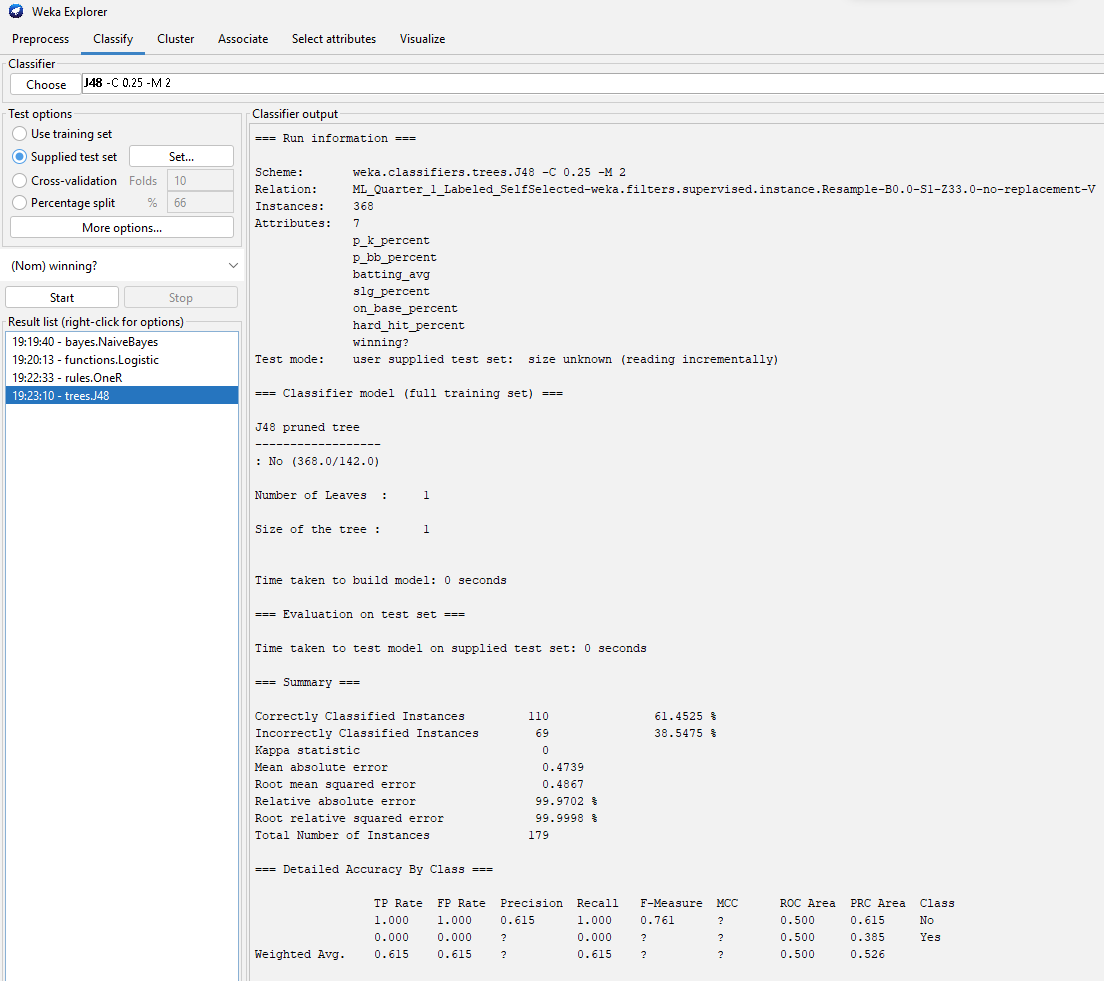
\includegraphics[scale=0.4]{./images/SelfSelected/J48.png}
\centering
    \caption{WEKA J48 Classification Results on SelfSelected Attributes}
    \label{fig:ssj48}
\end{figure}

\newpage 
\subsubsection{LogisticFunction - SelfSelected}
\begin{figure}[h!]
    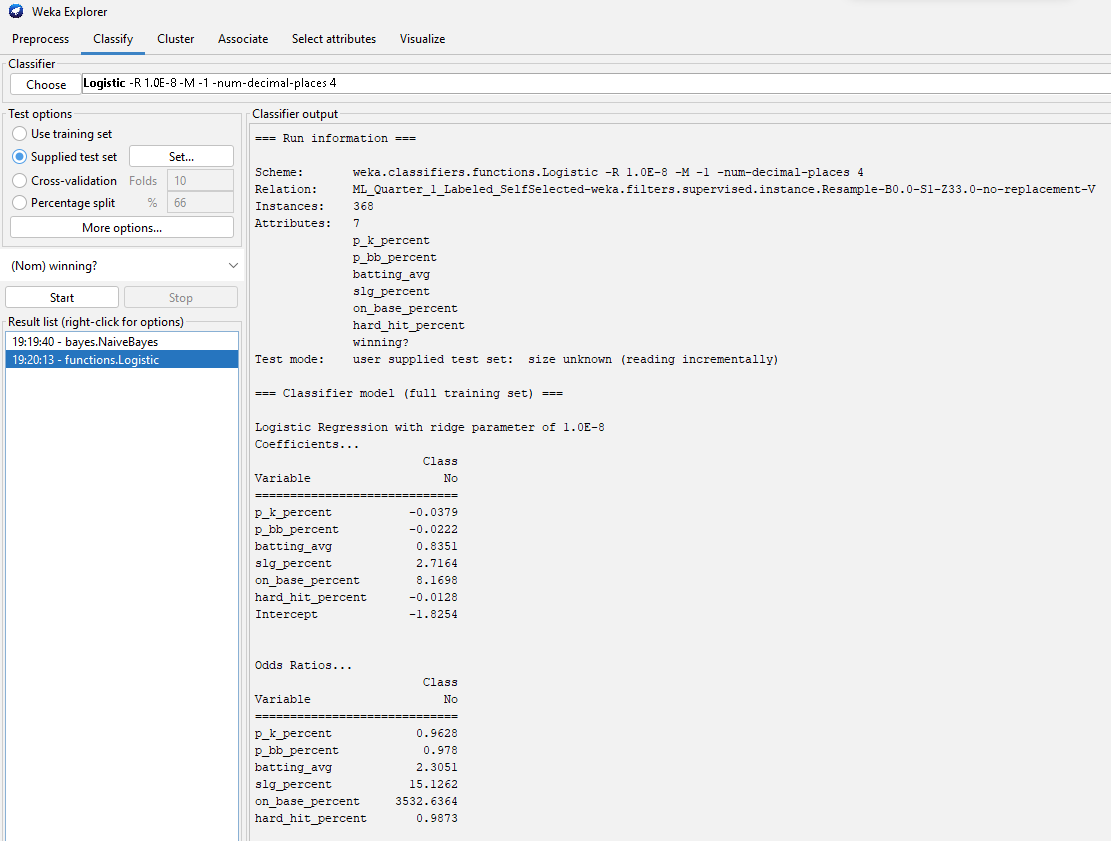
\includegraphics[scale=0.4]{./images/SelfSelected/LogisticFunction-Model.png}
\centering
    \caption{WEKA LogisticFunction Model on SelfSelected Attributes}
\end{figure}
\newpage
\begin{figure}[h!]
    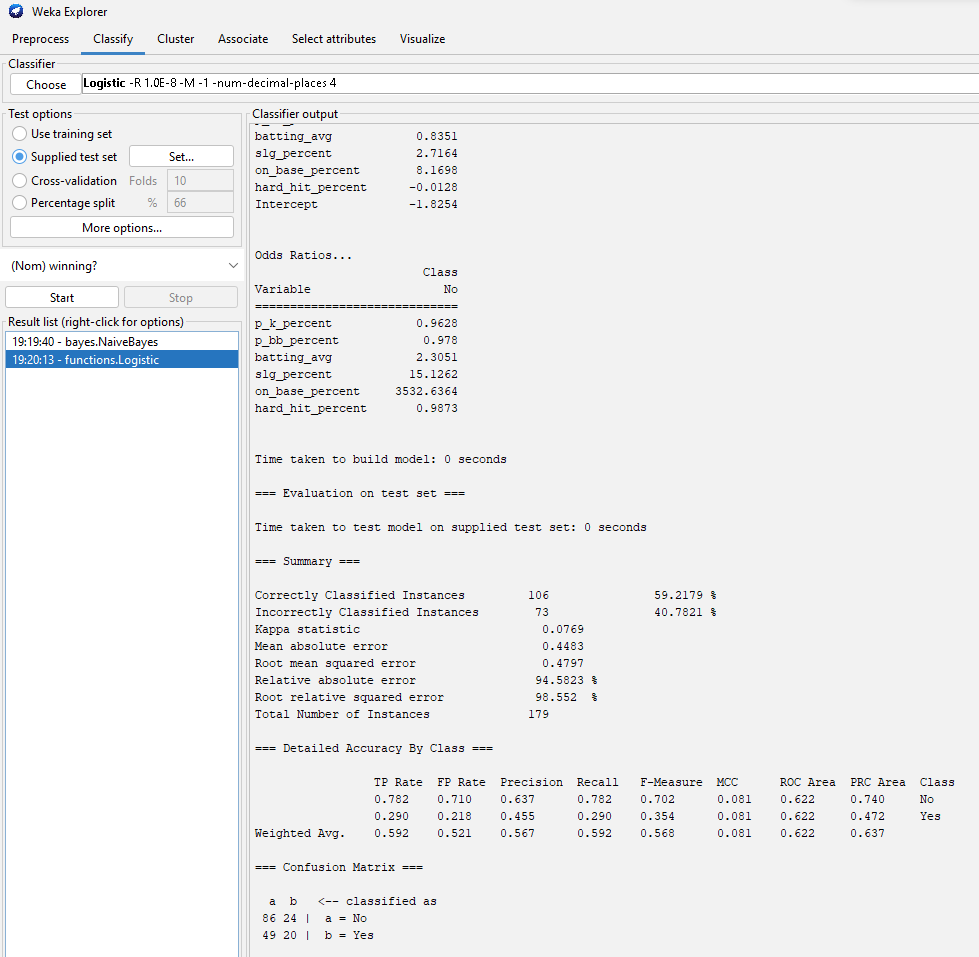
\includegraphics[scale=0.4]{./images/SelfSelected/LogisticFunction-Summary.png}
\centering
    \caption{WEKA LogisticFunction Summary Results on SelfSelected Attributes}
\end{figure}

\newpage
\subsubsection{NaiveBayes - SelfSelected}
\begin{figure}[h!]
    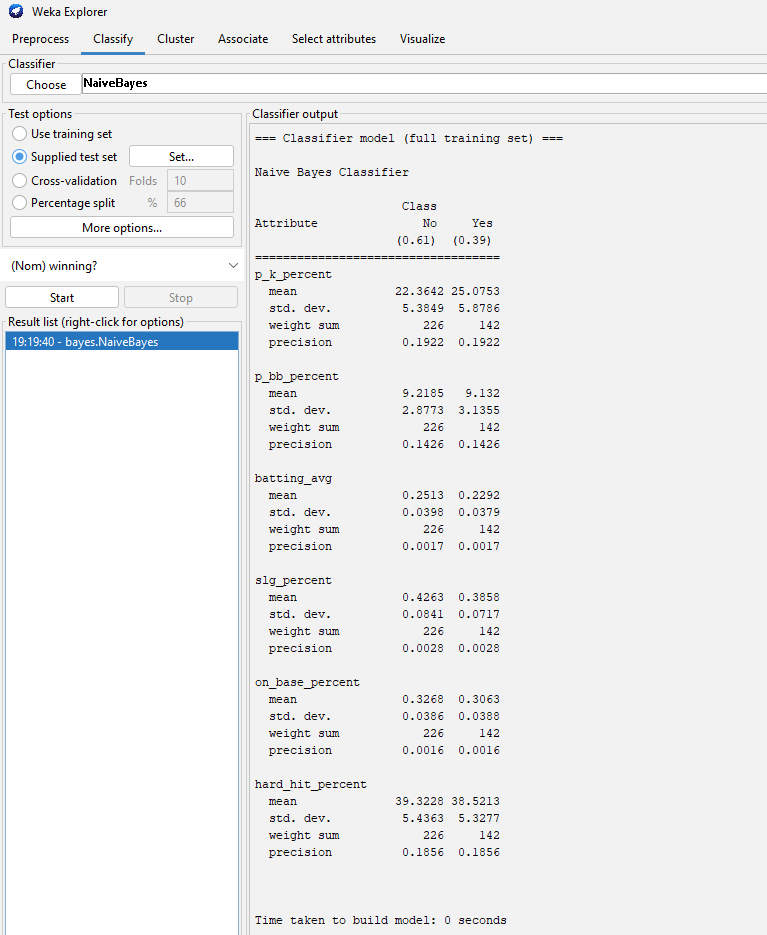
\includegraphics[scale=0.4]{./images/SelfSelected/NaiveBayes-Model.png}
\centering
    \caption{WEKA NaiveBayes Model on SelfSelected Attributes}
\end{figure}
\newpage
\begin{figure}[h!]
    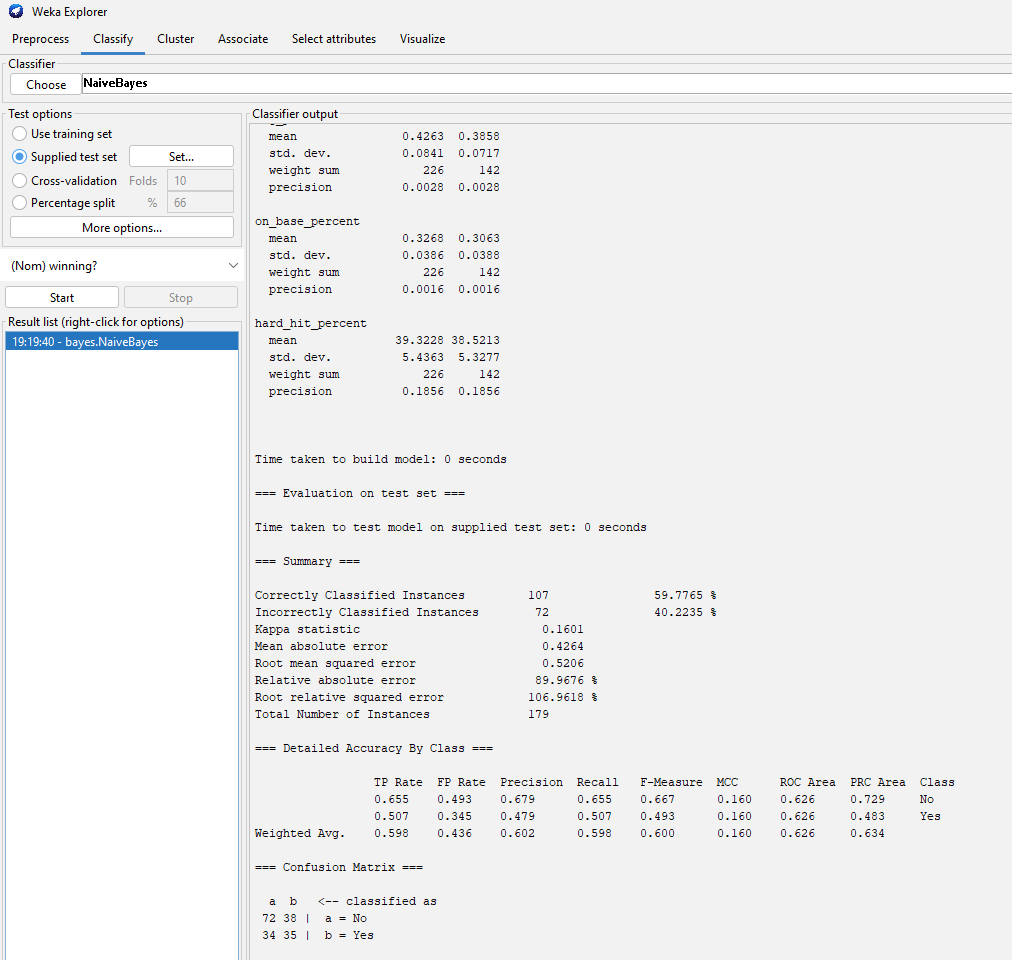
\includegraphics[scale=0.4]{./images/SelfSelected/NaiveBayes-Summary.png}
\centering
    \caption{WEKA NaiveBayes Summary Results on SelfSelected Attributes}
\end{figure}

\newpage
\subsubsection{OneR - SelfSelected}
\begin{figure}[h!]
    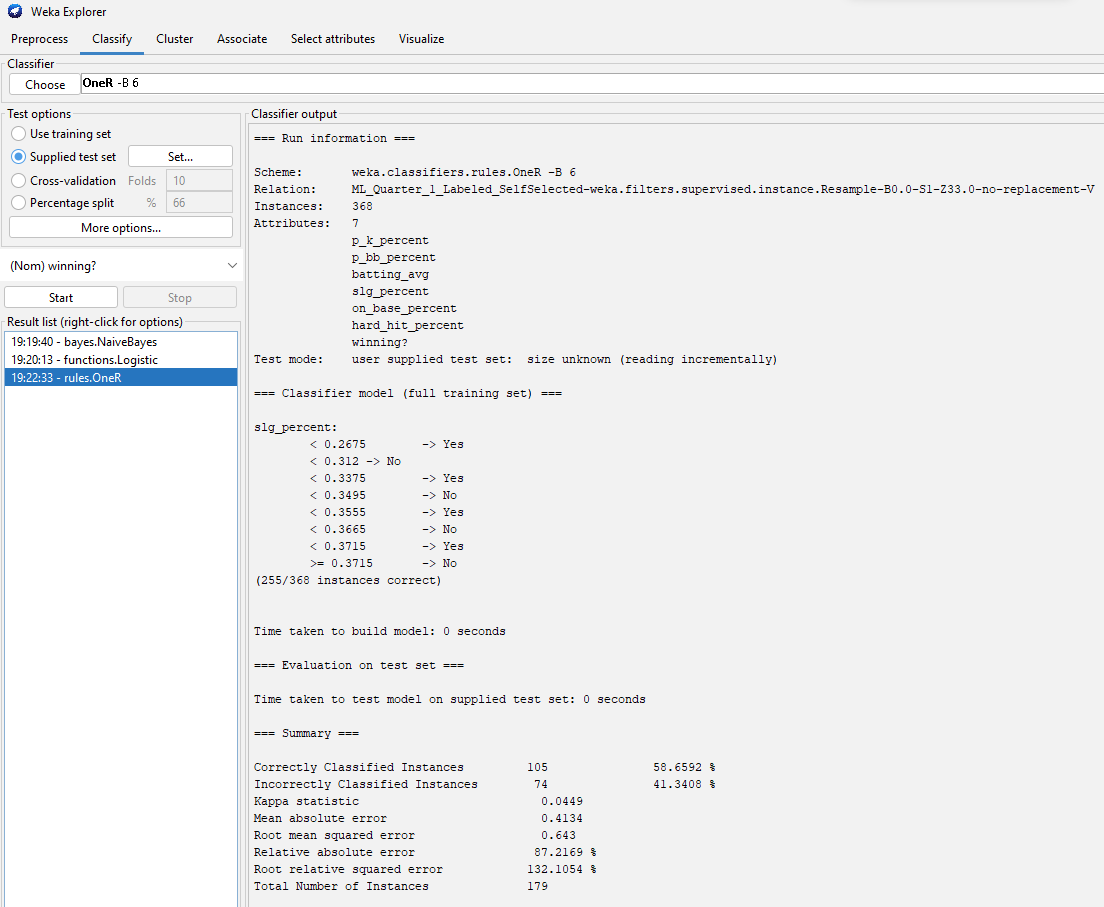
\includegraphics[scale=0.4]{./images/SelfSelected/OneR-Model.png}
\centering
    \caption{WEKA OneR Model on SelfSelected Attributes}
\end{figure}
\newpage
\begin{figure}[h!]
    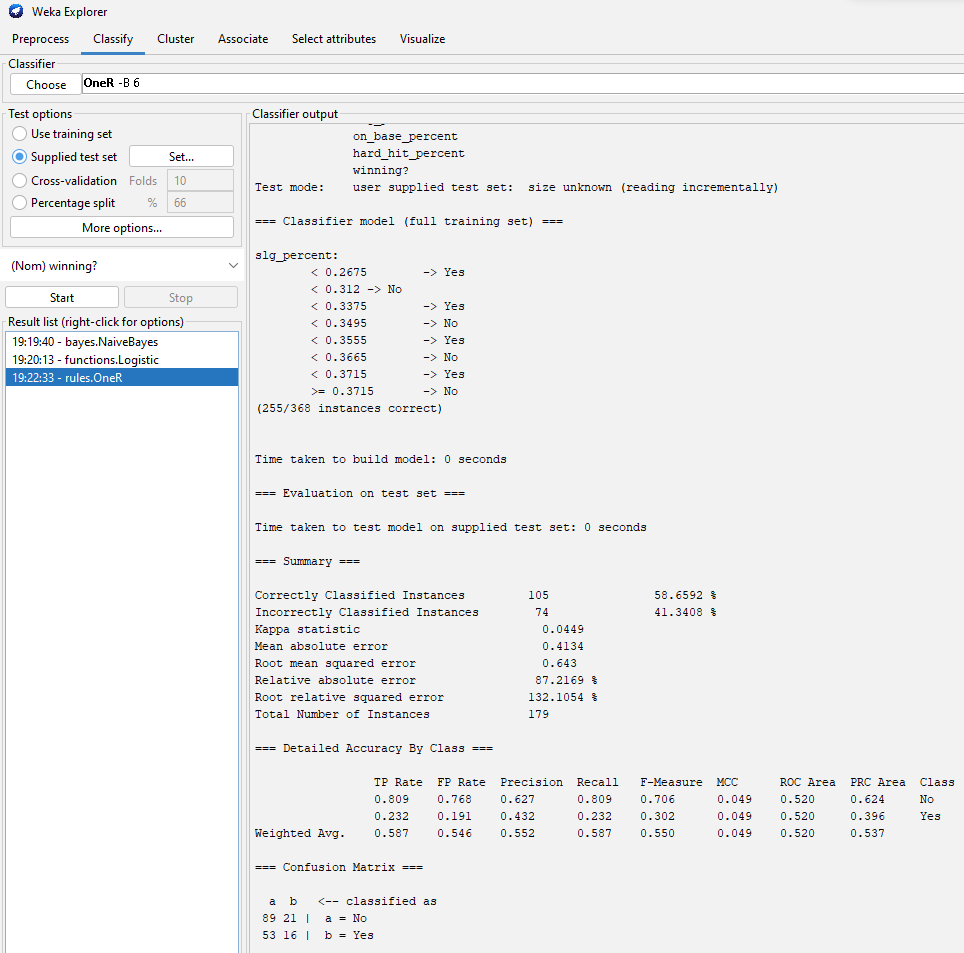
\includegraphics[scale=0.4]{./images/SelfSelected/OneR-Summary.png}
\centering
    \caption{WEKA OneR Summary Results on SelfSelected Attributes}
\end{figure}

\newpage
\subsubsection{Analysis}
We can see that overall $\textbf{J48}$ performed with the highest accuracy. However, one thing to note is that there are no true negatives for $\textbf{J48}$ classification. 

\newpage
\subsection{WrapperSubsetEval}

\subsubsection{J48 - WrapperSubsetEval}
\begin{figure}[h!]
    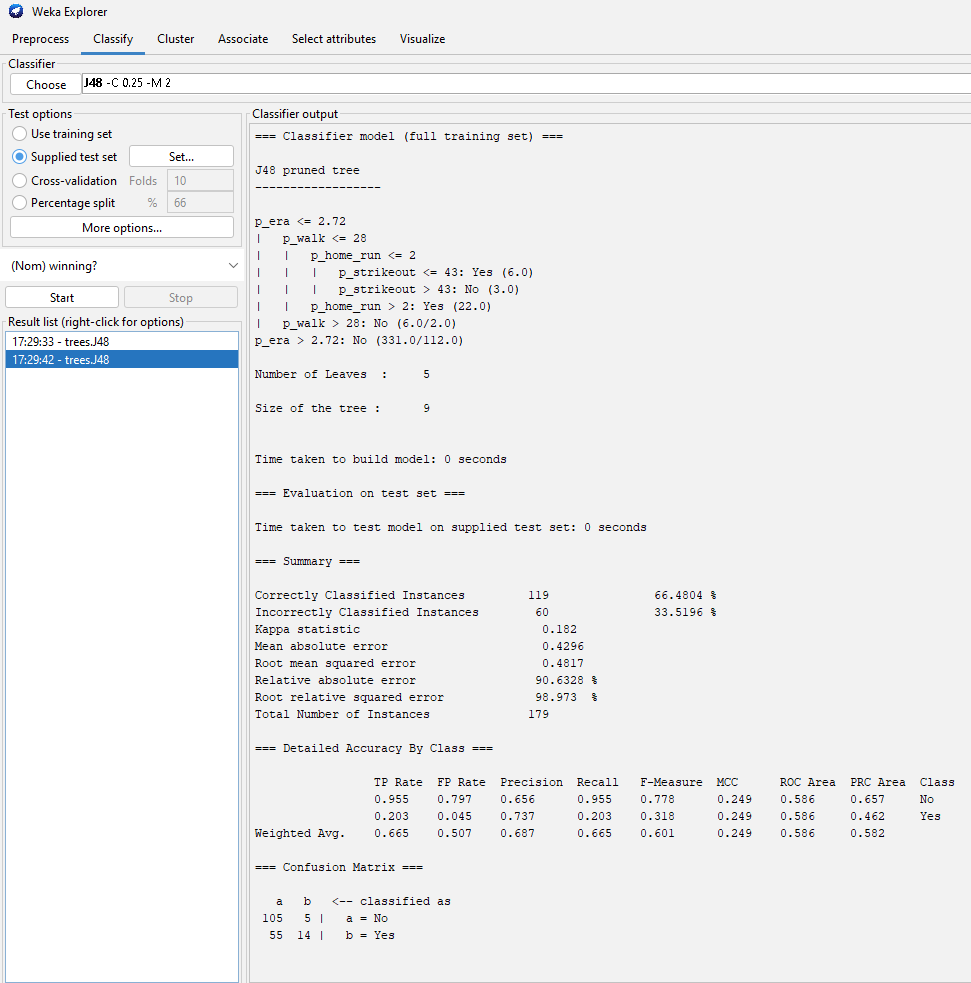
\includegraphics[scale=0.4]{./images/WrapperSubsetEval/J48.png}
\centering
    \caption{WEKA J48 Classification Results on WrapperSubsetEval Attributes}
\end{figure}

\newpage 
\subsubsection{LogisticFunction - WrapperSubsetEval}
\begin{figure}[h!]
    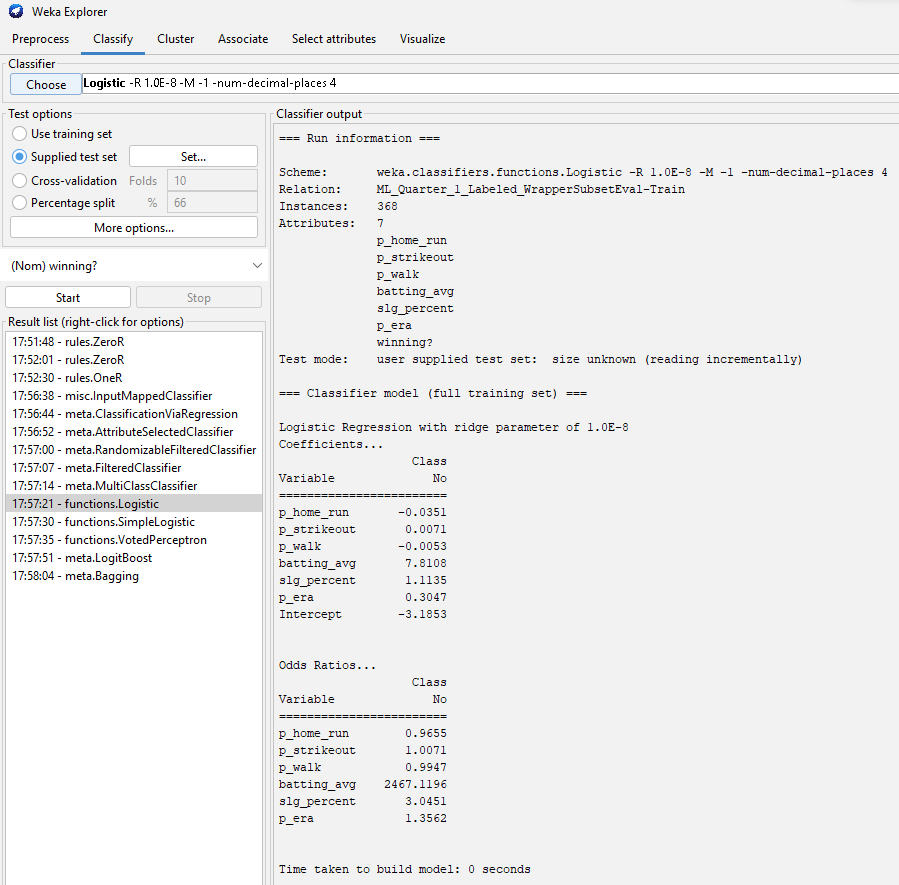
\includegraphics[scale=0.4]{./images/WrapperSubsetEval/LogisticFunction-Model.png}
\centering
    \caption{WEKA LogisticFunction Model on WrapperSubsetEval Attributes}
\end{figure}
\newpage
\begin{figure}[h!]
    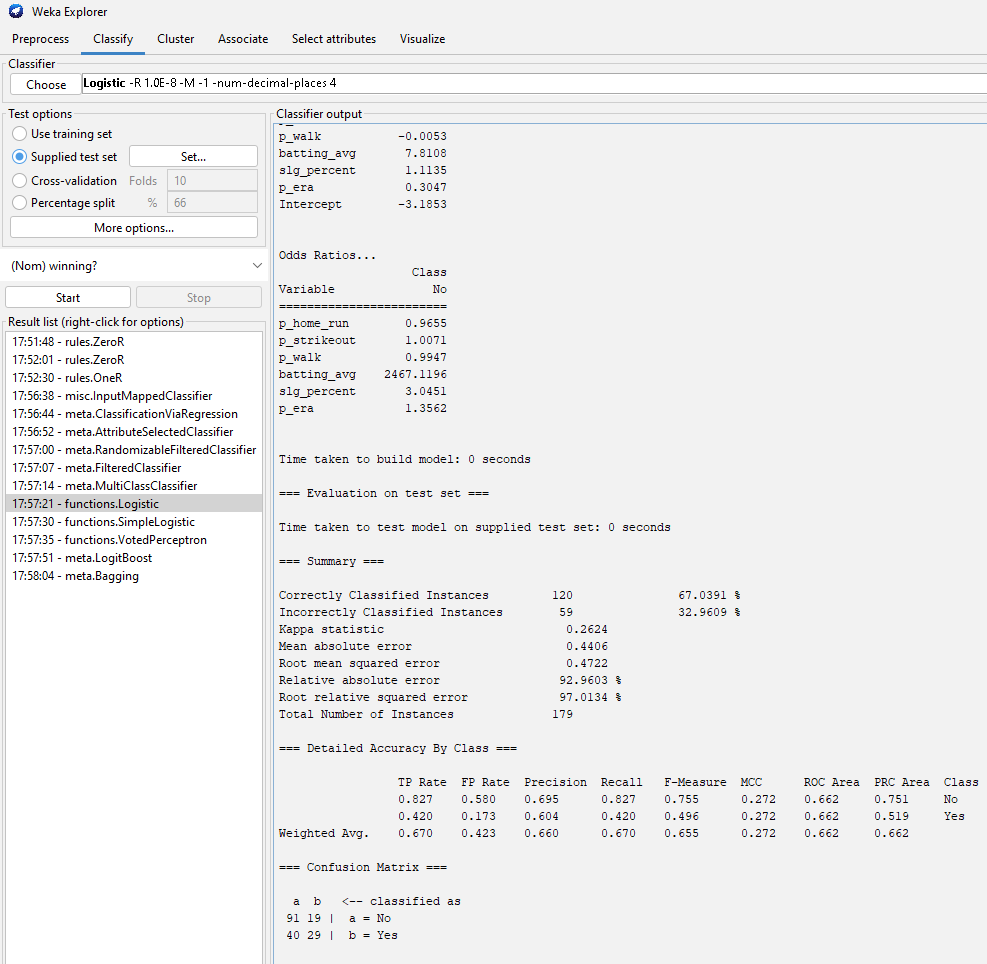
\includegraphics[scale=0.4]{./images/WrapperSubsetEval/LogisticFunction-Summary.png}
\centering
    \caption{WEKA LogisticFunction Summary Results on WrapperSubsetEval Attributes}
\end{figure}

\newpage
\subsubsection{NaiveBayes - WrapperSubsetEval}
\begin{figure}[h!]
    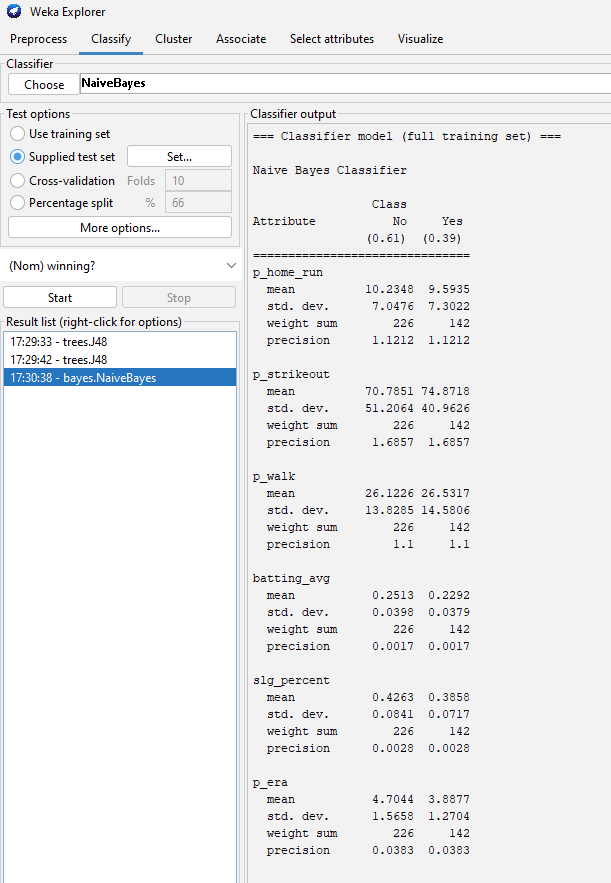
\includegraphics[scale=0.4]{./images/WrapperSubsetEval/NaiveBayes-Model.png}
\centering
    \caption{WEKA NaiveBayes Model on WrapperSubsetEval Attributes}
\end{figure}
\newpage
\begin{figure}[h!]
    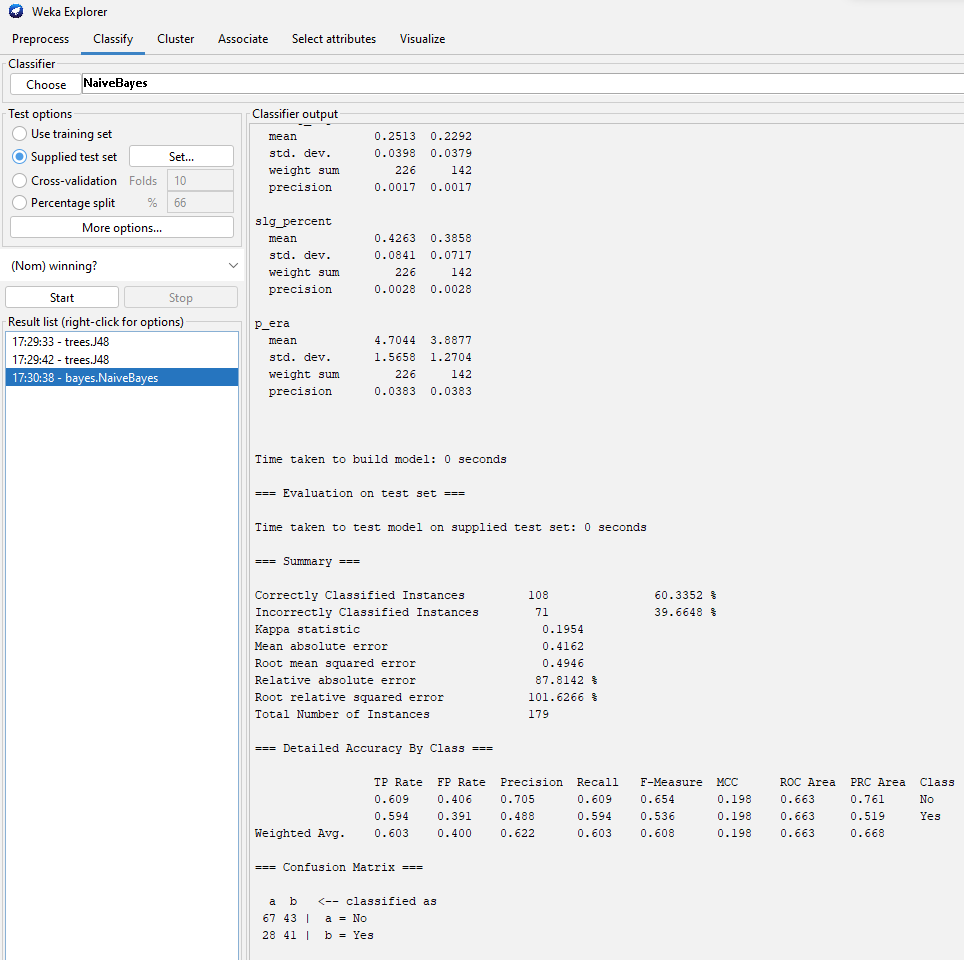
\includegraphics[scale=0.4]{./images/WrapperSubsetEval/NaiveBayes-Summary.png}
\centering
    \caption{WEKA NaiveBayes Summary Results on WrapperSubsetEval Attributes}
\end{figure}

\newpage
\subsubsection{OneR - WrapperSubsetEval}
\begin{figure}[h!]
    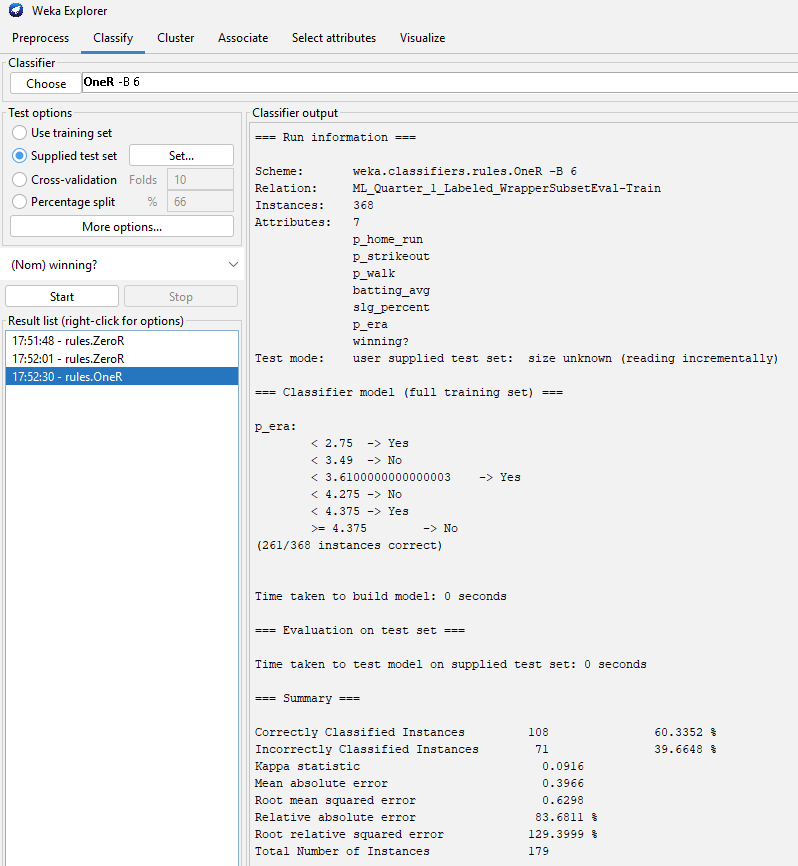
\includegraphics[scale=0.4]{./images/WrapperSubsetEval/OneR-Model.png}
\centering
    \caption{WEKA OneR Model on WrapperSubsetEval Attributes}
\end{figure}
\newpage
\begin{figure}[h!]
    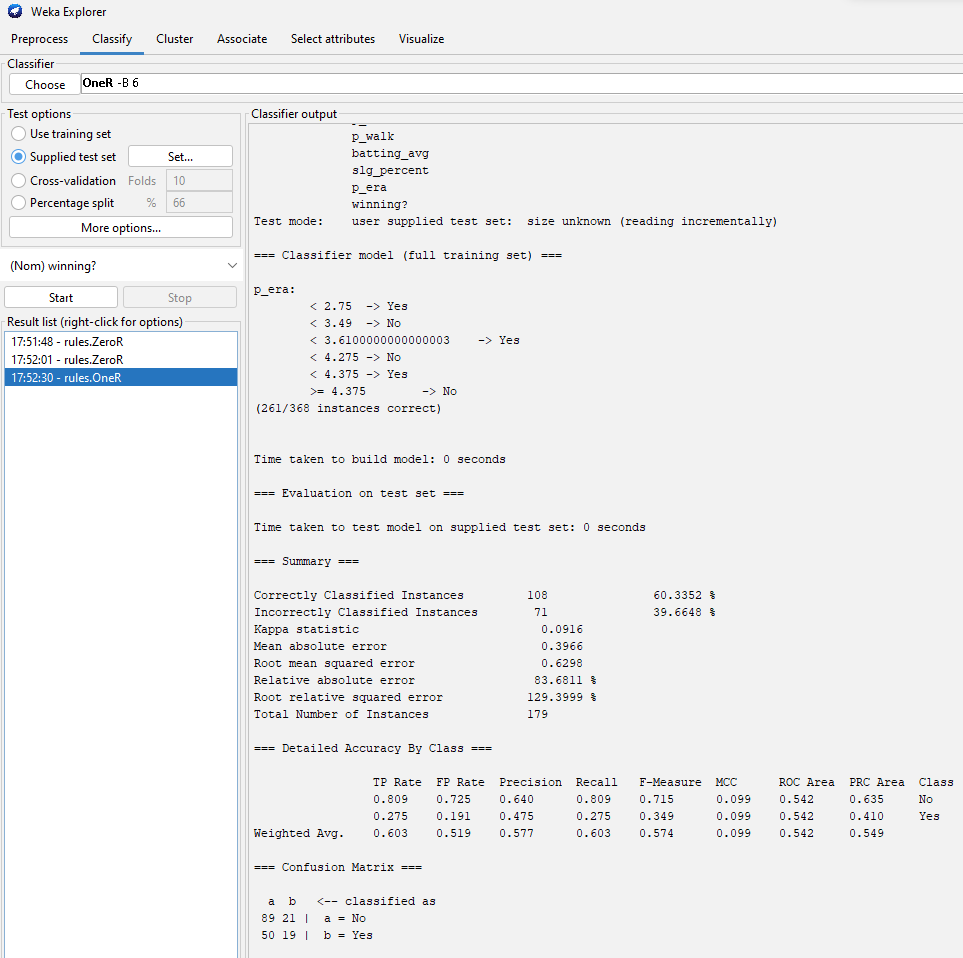
\includegraphics[scale=0.4]{./images/WrapperSubsetEval/OneR-Summary.png}
\centering
    \caption{WEKA OneR Summary Results on WrapperSubsetEval Attributes}
\end{figure}

\newpage
\subsubsection{Analysis}
We see that $\textbf{LogisticFunction}$ performed best here, but $\textbf{J48}$ was a close second with only one more instance misclassified. $\textbf{J48}$ was a lot better at determining true positives while $\textbf{LogisticFunction}$ was a lot better at determining true negatives. 


\newpage
\subsection{InfoGainAttributeEval}

\subsubsection{J48 - InfoGainAttributeEval}
\begin{figure}[h!]
    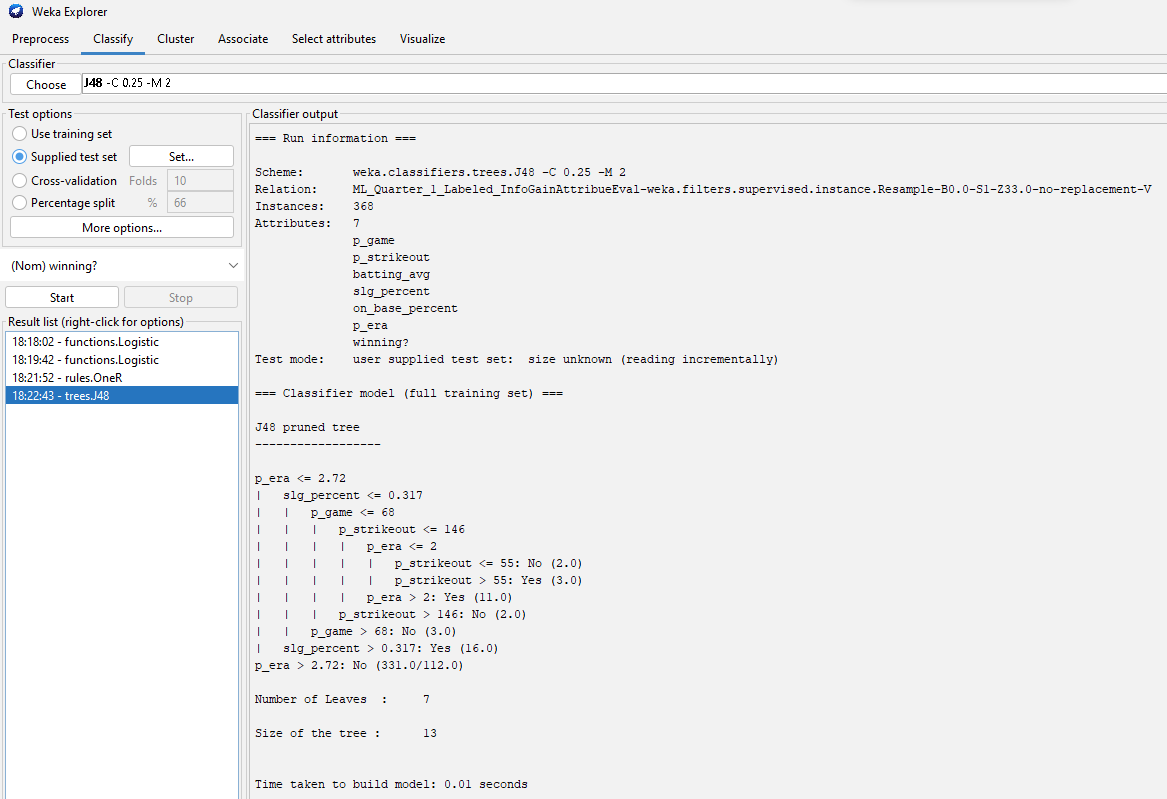
\includegraphics[scale=0.4]{./images/InfoGainAttributeEval/J48-Model.png}
\centering
    \caption{WEKA J48 Model on InfoGainAttributeEval Attributes}
\end{figure}
\newpage
\begin{figure}[h!]
    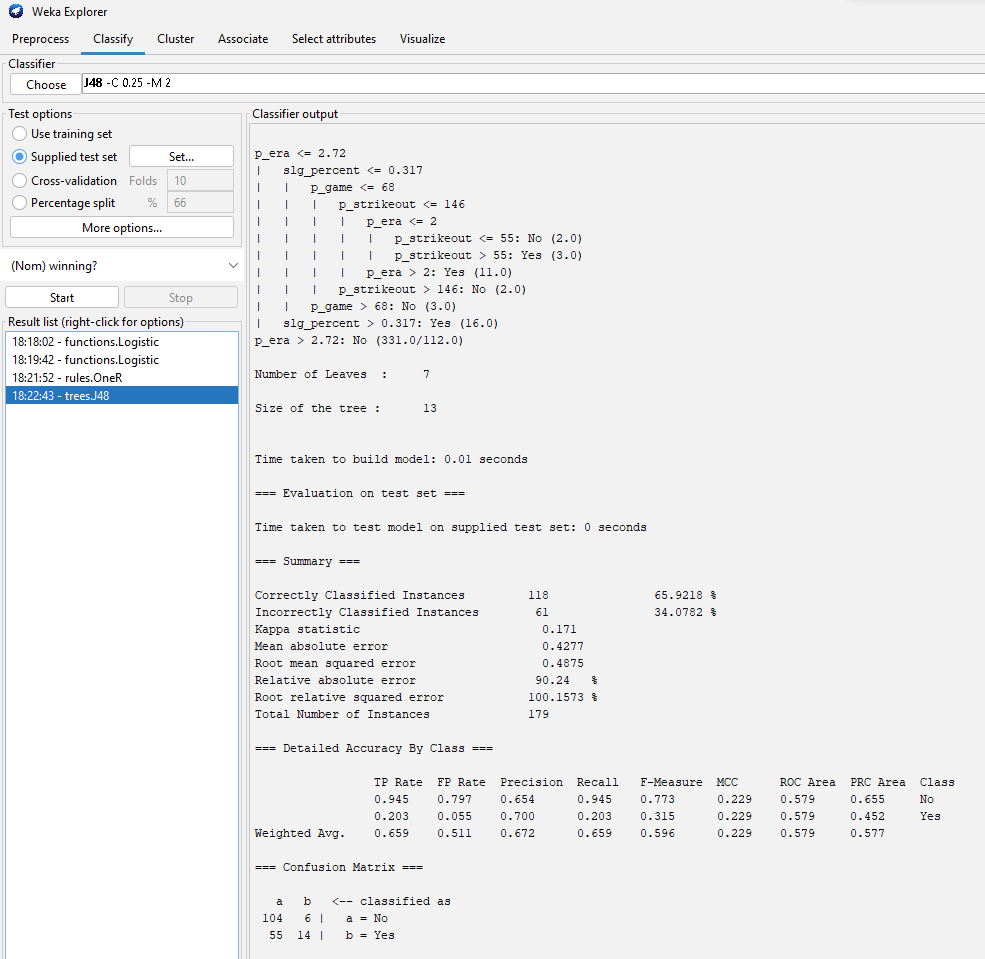
\includegraphics[scale=0.4]{./images/InfoGainAttributeEval/J48-Summary.png}
\centering
    \caption{WEKA J48 Classification Results on InfoGainAttributeEval Attributes}
\end{figure}

\newpage 
\subsubsection{LogisticFunction - InfoGainAttributeEval}
\begin{figure}[h!]
    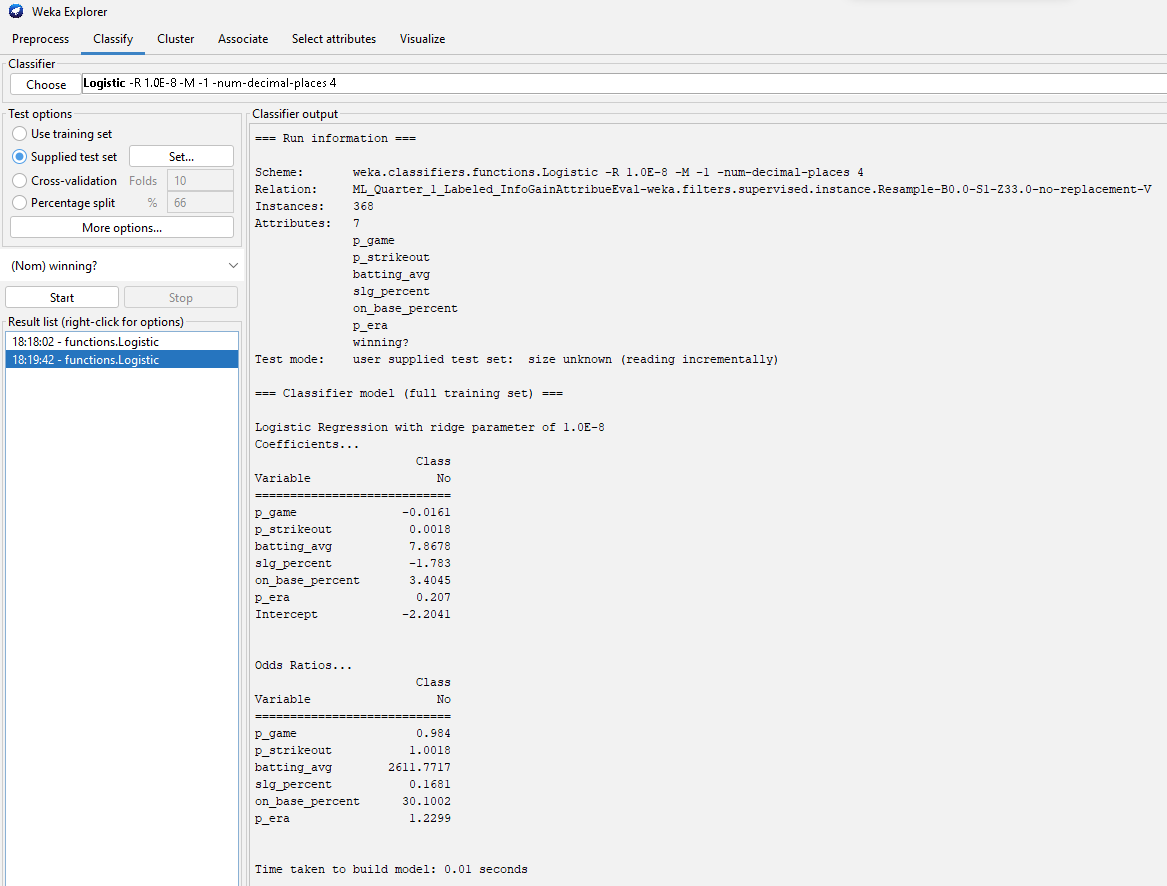
\includegraphics[scale=0.4]{./images/InfoGainAttributeEval/LogisticFunction-Model.png}
\centering
    \caption{WEKA LogisticFunction Model on InfoGainAttributeEval Attributes}
\end{figure}
\newpage
\begin{figure}[h!]
    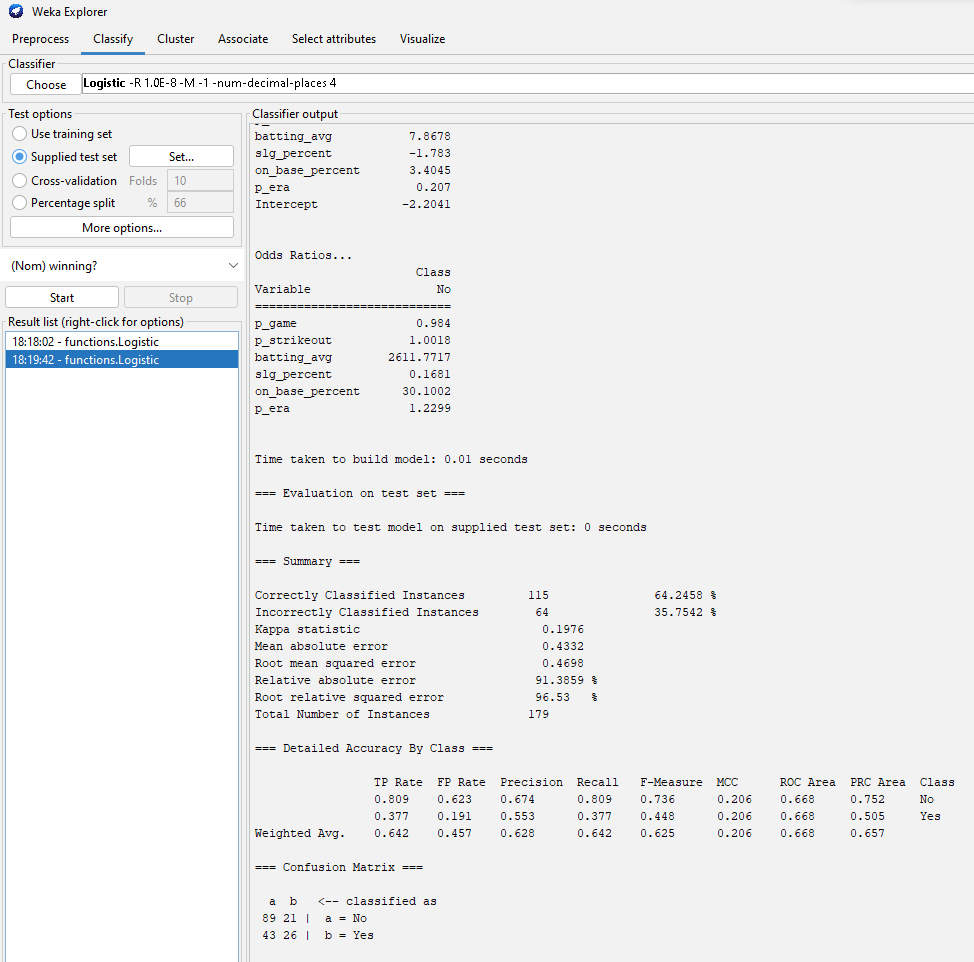
\includegraphics[scale=0.4]{./images/InfoGainAttributeEval/LogisticFunction-Summary.png}
\centering
    \caption{WEKA LogisticFunction Summary Results on InfoGainAttributeEval Attributes}
\end{figure}
\newpage
\subsubsection{NaiveBayes - InfoGainAttributeEval}
\begin{figure}[h!]
    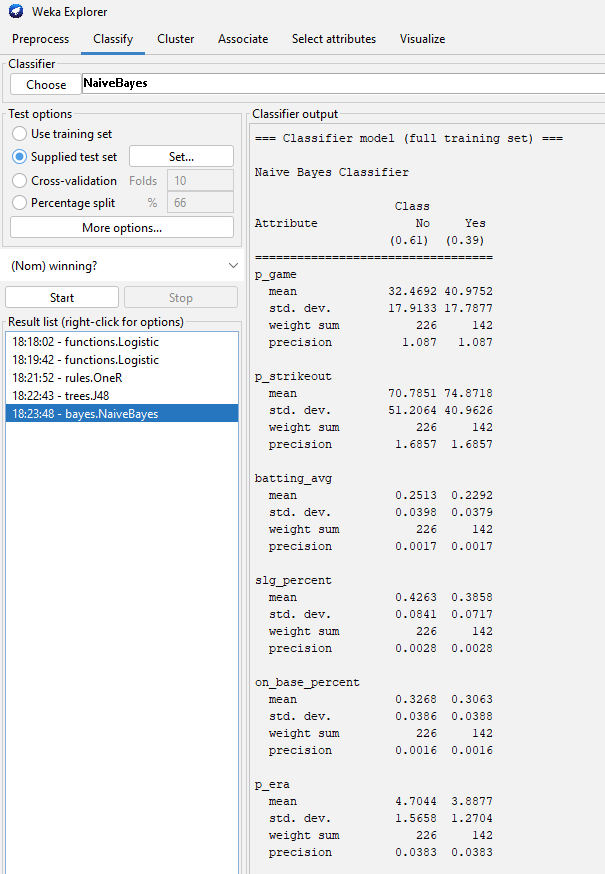
\includegraphics[scale=0.4]{./images/InfoGainAttributeEval/NaiveBayes-Model.png}
\centering
    \caption{WEKA NaiveBayes Model on InfoGainAttributeEval Attributes}
\end{figure}
\newpage
\begin{figure}[h!]
    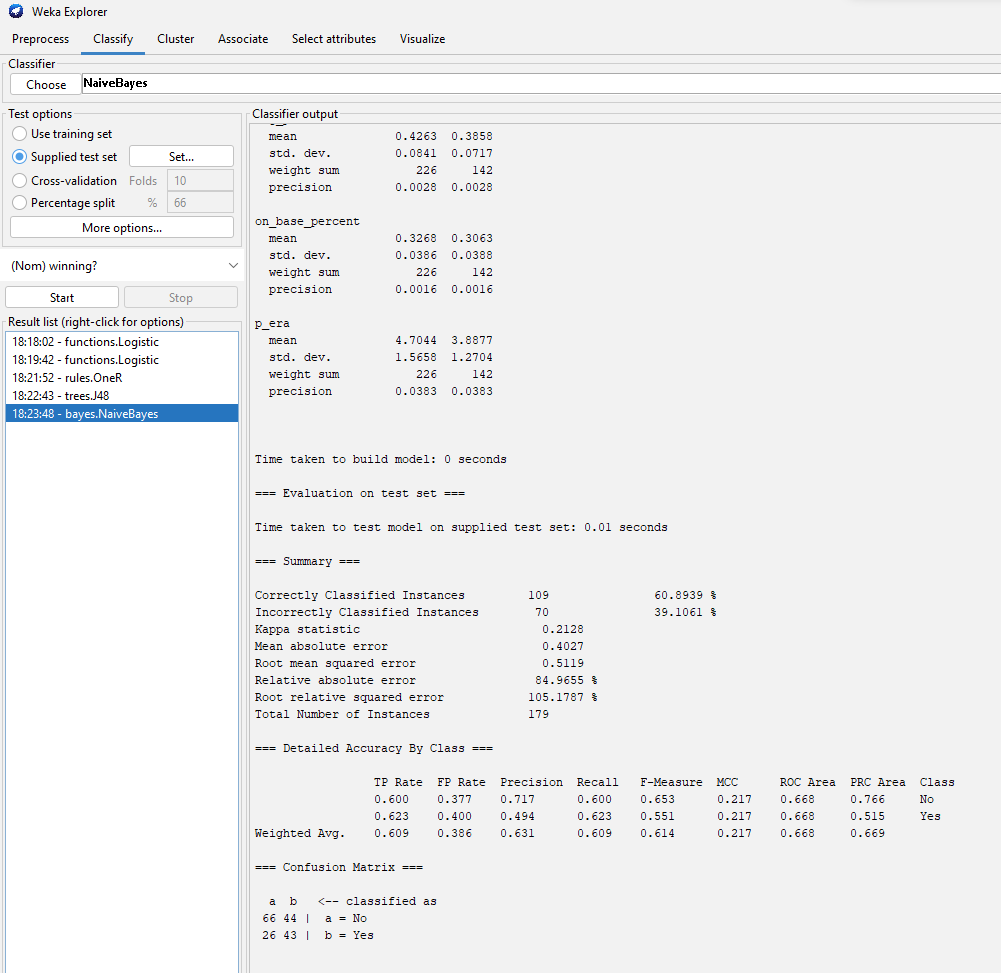
\includegraphics[scale=0.4]{./images/InfoGainAttributeEval/NaiveBayes-Summary.png}
\centering
    \caption{WEKA NaiveBayes Summary Results on InfoGainAttributeEval Attributes}
\end{figure}

\newpage
\subsubsection{OneR - InfoGainAttributeEval}
\begin{figure}[h!]
    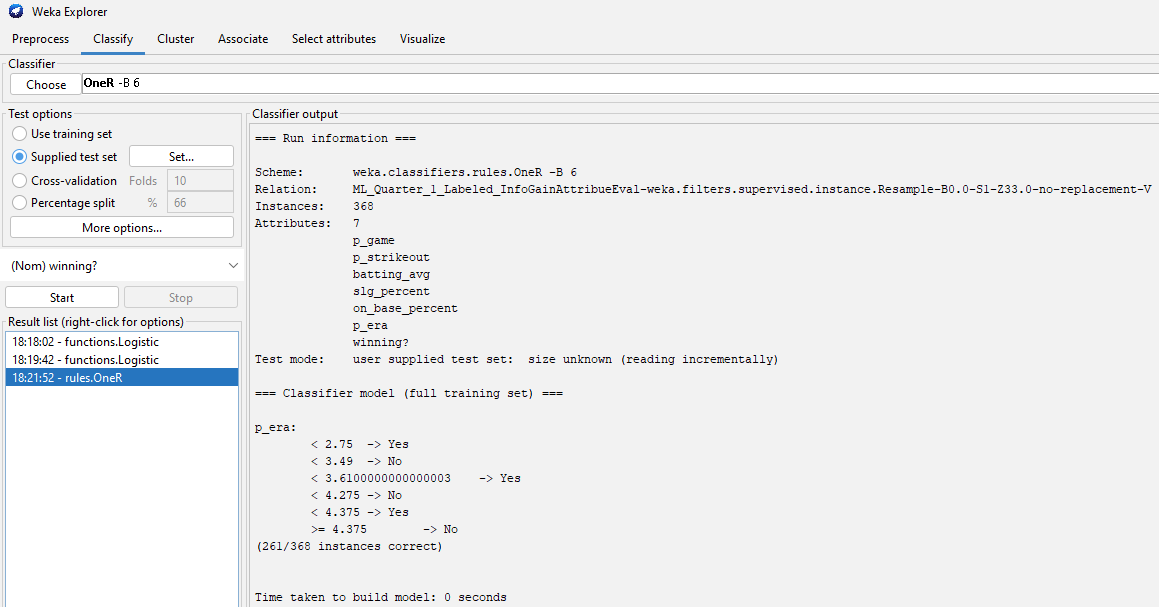
\includegraphics[scale=0.4]{./images/InfoGainAttributeEval/OneR-Model.png}
\centering
    \caption{WEKA OneR Model on InfoGainAttributeEval Attributes}
\end{figure}
\newpage
\begin{figure}[h!]
    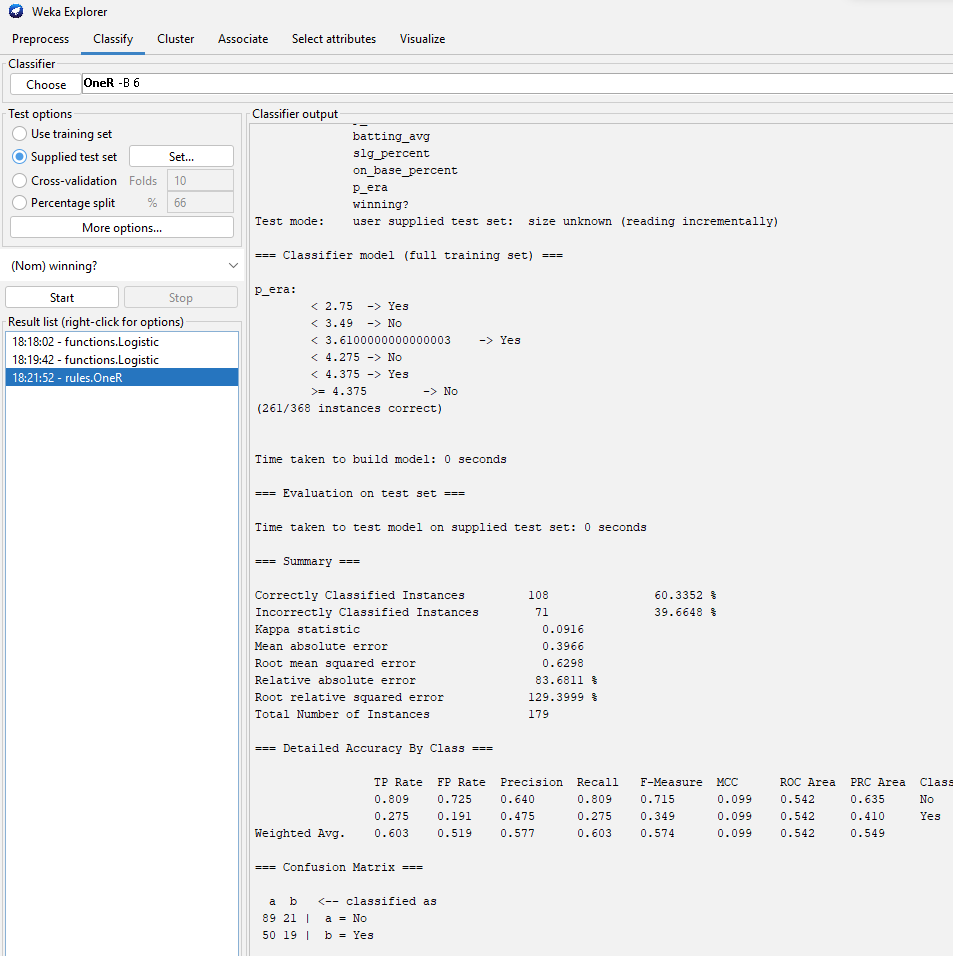
\includegraphics[scale=0.4]{./images/InfoGainAttributeEval/OneR-Summary.png}
\centering
    \caption{WEKA OneR Summary Results on InfoGainAttributeEval Attributes}
\end{figure}

\newpage
\subsubsection{Analysis}
$\textbf{J48}$ performed the best with this attribute selection method, with $\textbf{LogisticFunction}$ being a close scond. Once again, $\textbf{J48}$ was a lot better at categorizing true positives while $\textbf{LogisticFunction}$ was a lot better at categorizing true negatives. 


\newpage
\subsection{GainRatioAttributeEval}

\subsubsection{J48 - GainRatioAttributeEval}
\begin{figure}[h!]
    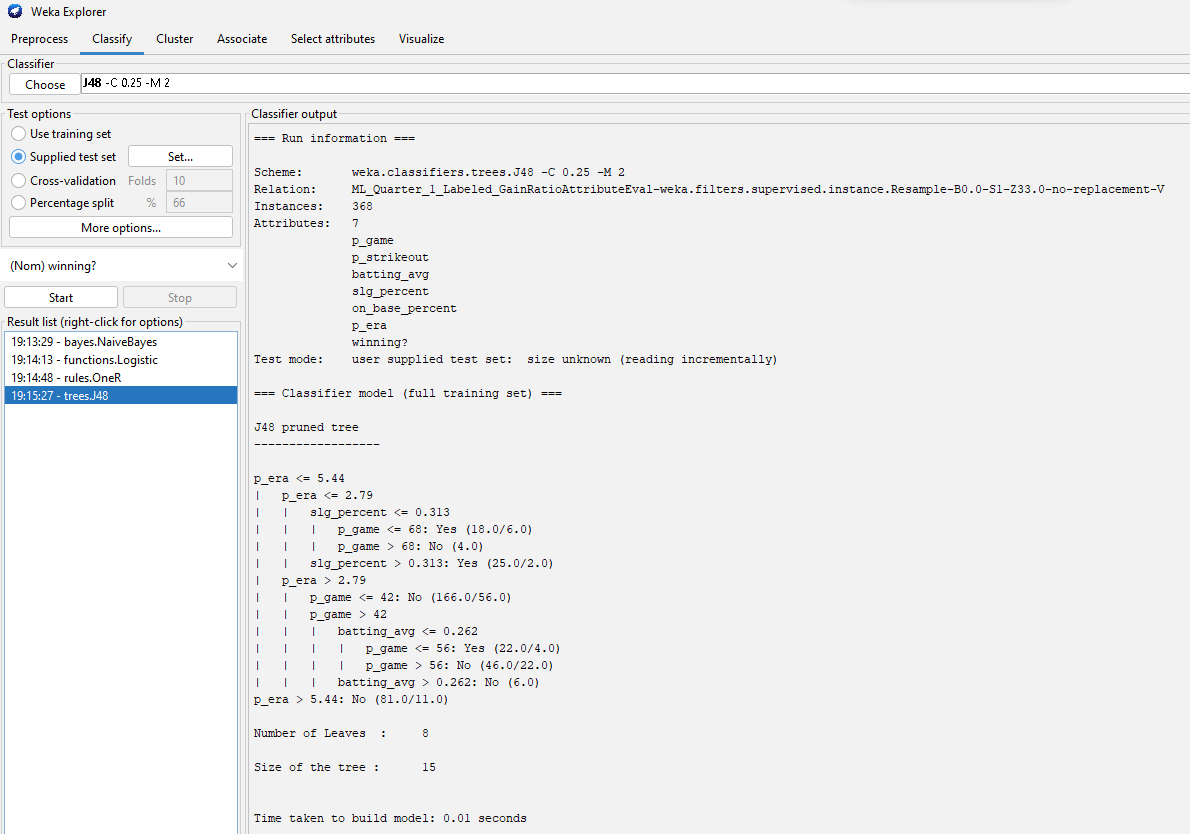
\includegraphics[scale=0.4]{./images/GainRatioAttributeEval/J48-Model.png}
\centering
    \caption{WEKA J48 Model on GainRatioAttributeEval Attributes}
\end{figure}
\newpage
\begin{figure}[h!]
    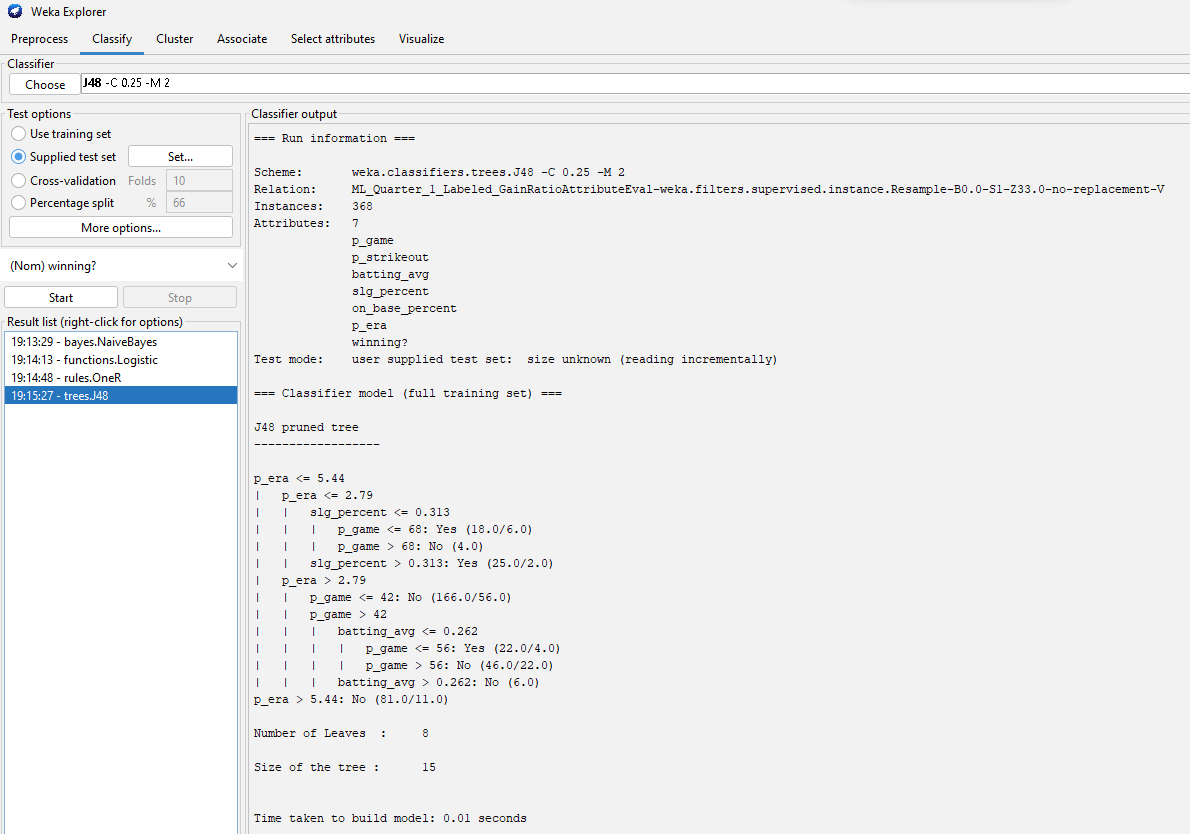
\includegraphics[scale=0.4]{./images/GainRatioAttributeEval/J48-Model.png}
\centering
    \caption{WEKA J48 Classification Results on GainRatioAttributeEval Attributes}
\end{figure}

\newpage 
\subsubsection{LogisticFunction - GainRatioAttributeEval}
\begin{figure}[h!]
    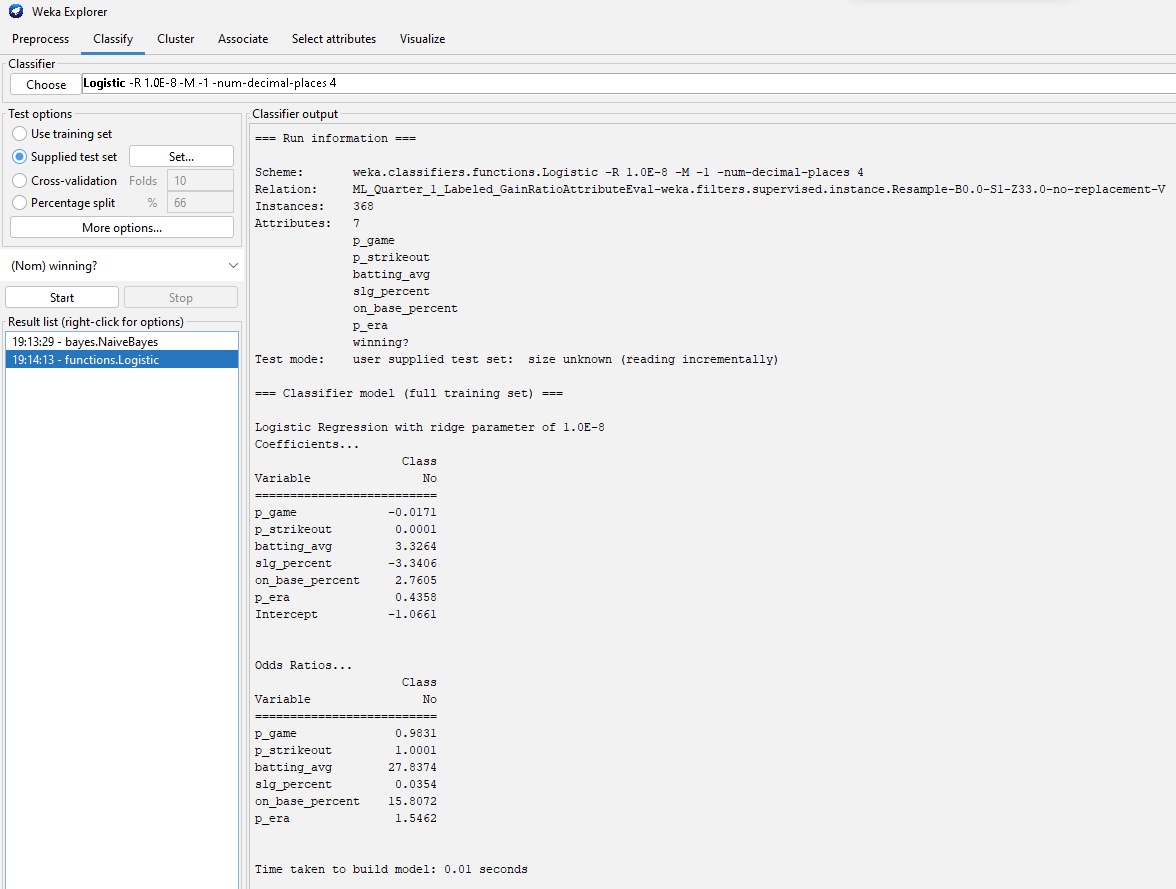
\includegraphics[scale=0.4]{./images/GainRatioAttributeEval/LogisticFunction-Model.png}
\centering
    \caption{WEKA LogisticFunction Model on GainRatioAttributeEval Attributes}
\end{figure}
\newpage
\begin{figure}[h!]
    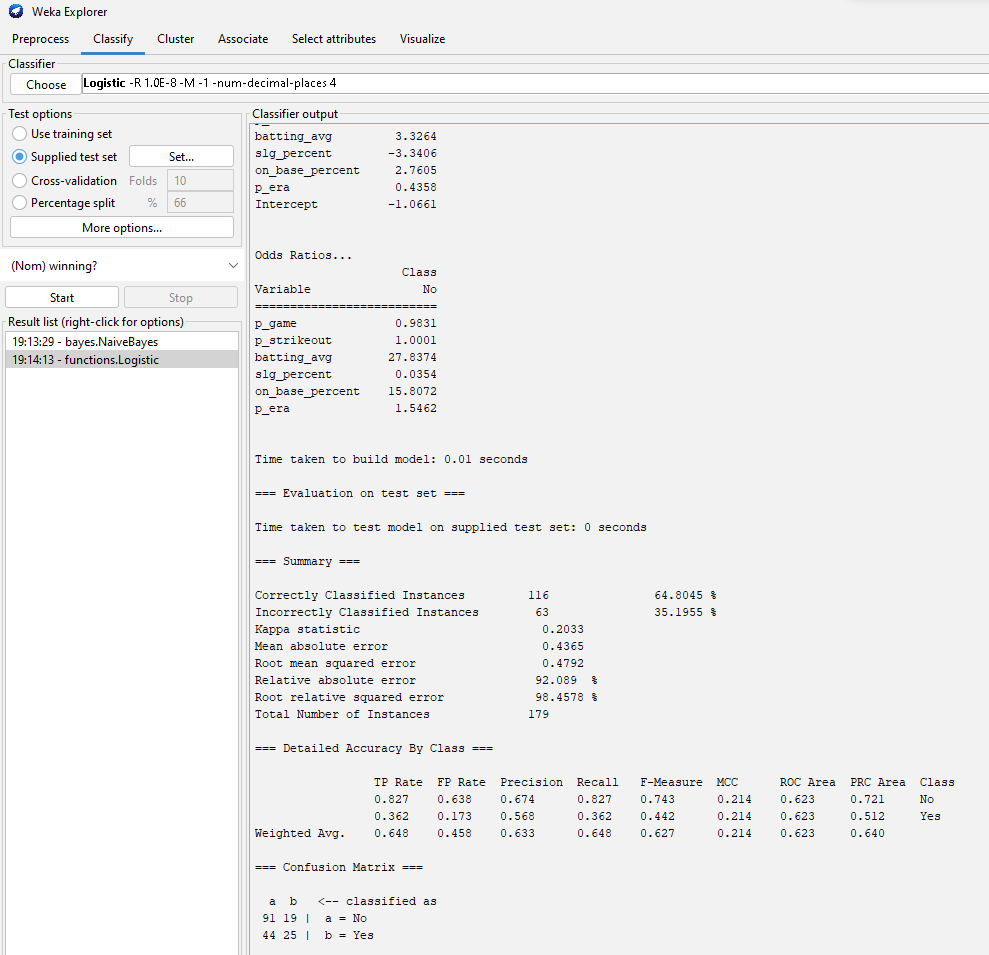
\includegraphics[scale=0.4]{./images/GainRatioAttributeEval/LogisticFunction-Summary.png}
\centering
    \caption{WEKA LogisticFunction Summary Results on GainRatioAttributeEval Attributes}
\end{figure}

\newpage
\subsubsection{NaiveBayes - GainRatioAttributeEval}
\begin{figure}[h!]
    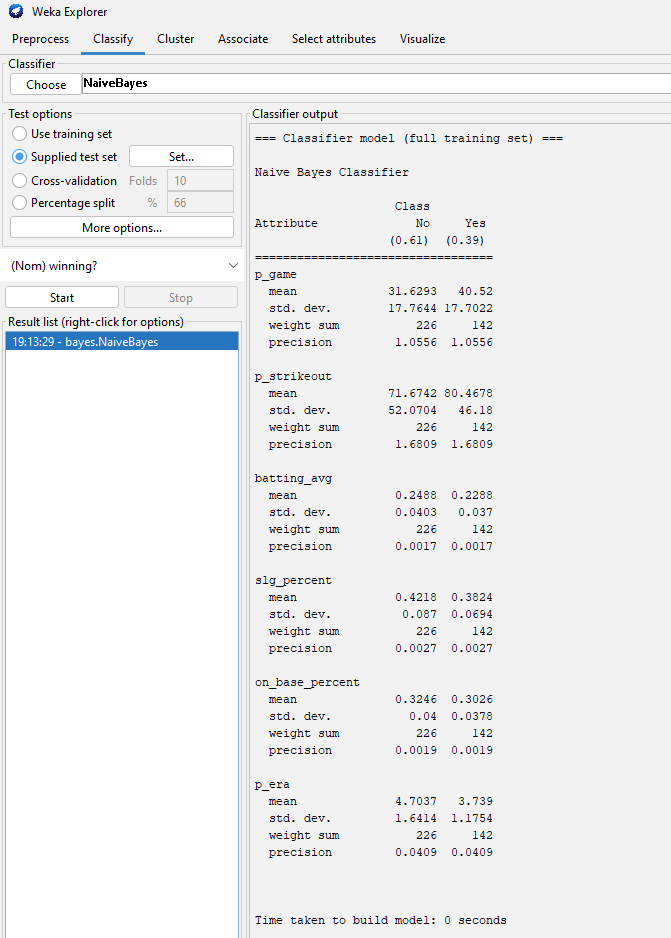
\includegraphics[scale=0.4]{./images/GainRatioAttributeEval/NaiveBayes-Model.png}
\centering
    \caption{WEKA NaiveBayes Model on GainRatioAttributeEval Attributes}
\end{figure}
\newpage
\begin{figure}[h!]
    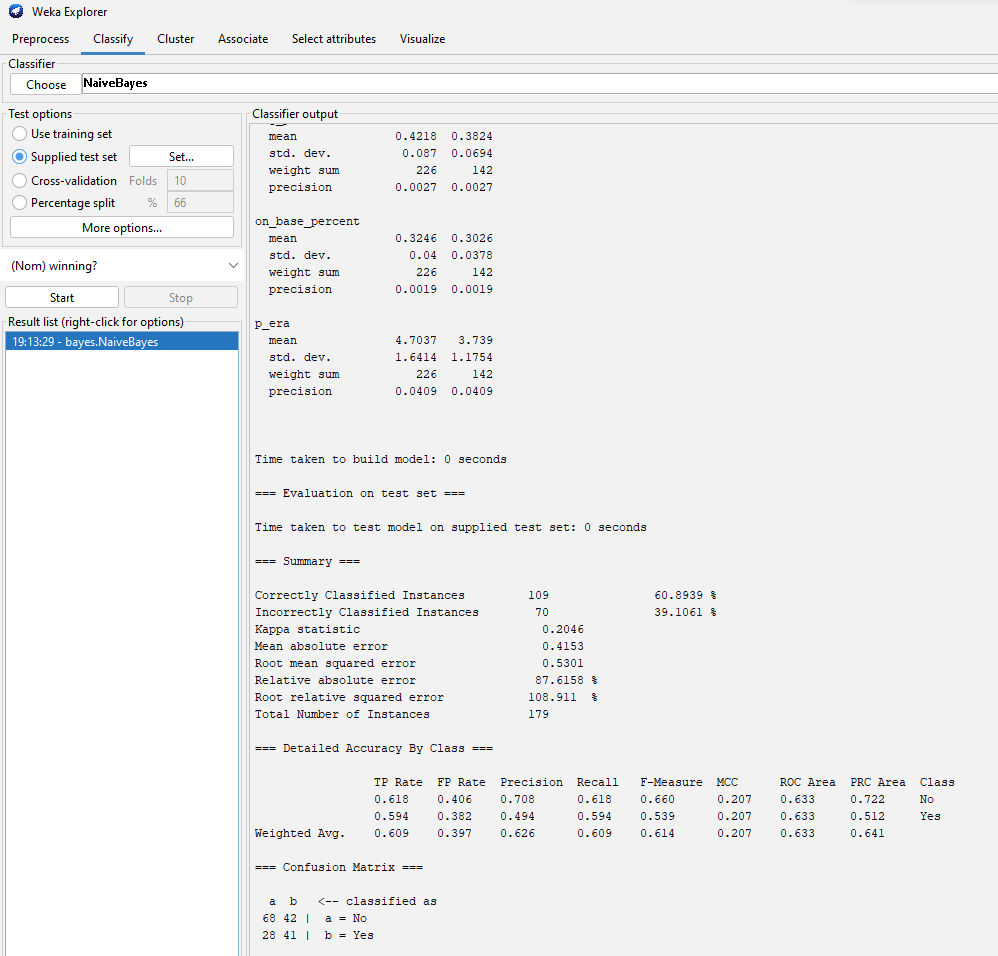
\includegraphics[scale=0.4]{./images/GainRatioAttributeEval/NaiveBayes-Summary.png}
\centering
    \caption{WEKA NaiveBayes Summary Results on GainRatioAttributeEval Attributes}
\end{figure}

\newpage
\subsubsection{OneR - GainRatioAttributeEval}
\begin{figure}[h!]
    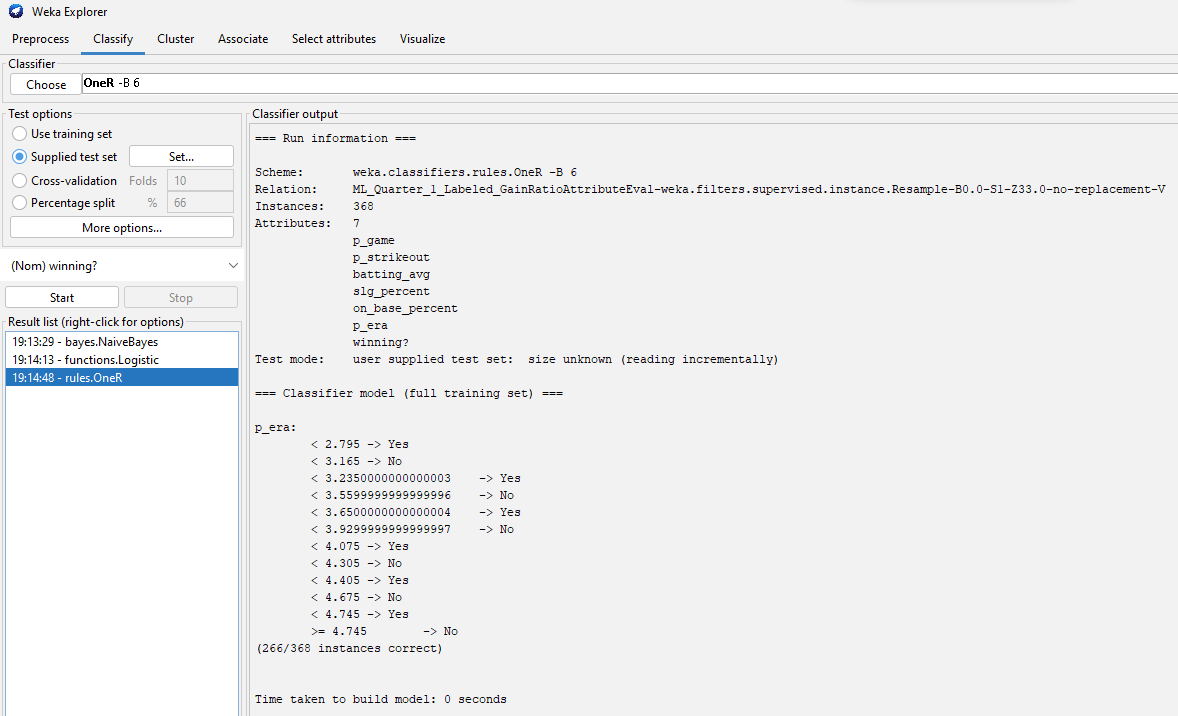
\includegraphics[scale=0.4]{./images/GainRatioAttributeEval/OneR-Model.png}
\centering
    \caption{WEKA OneR Model on GainRatioAttributeEval Attributes}
\end{figure}
\newpage
\begin{figure}[h!]
    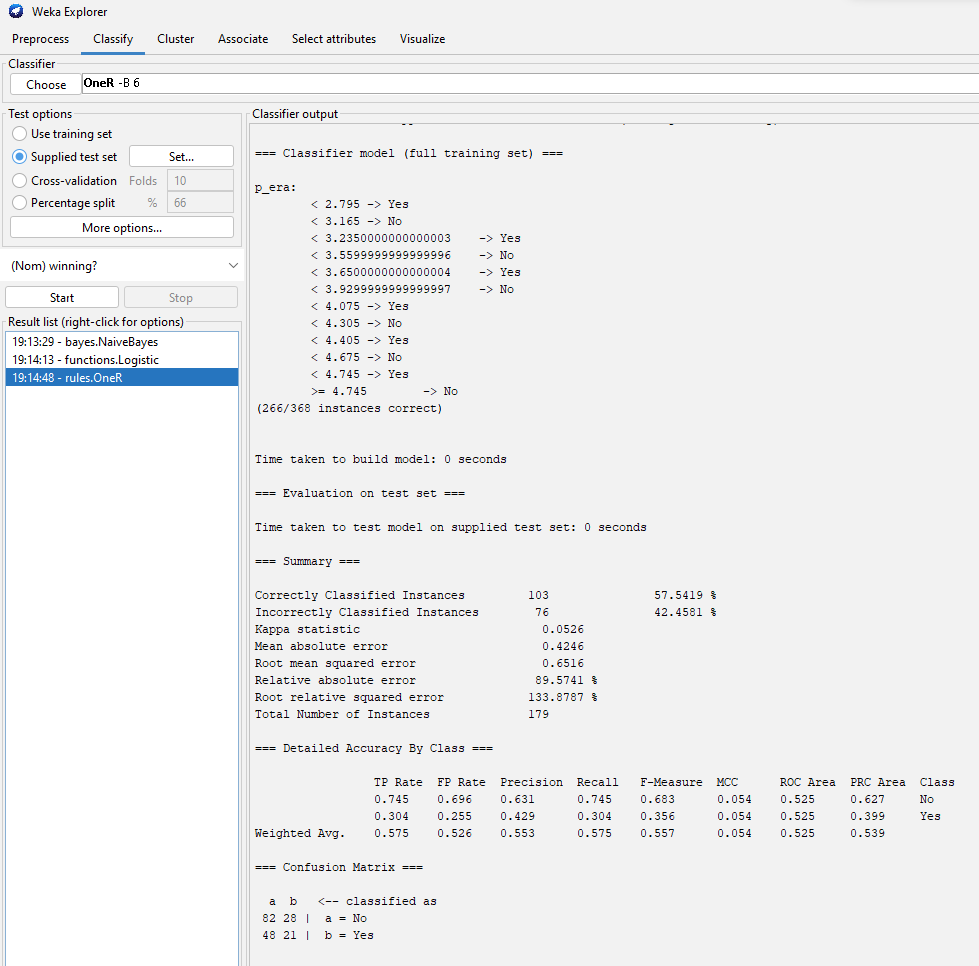
\includegraphics[scale=0.4]{./images/GainRatioAttributeEval/OneR-Summary.png}
\centering
    \caption{WEKA OneR Summary Results on GainRatioAttributeEval Attributes}
\end{figure}

\newpage
\subsubsection{Analysis}
$\textbf{J48}$ performed the best with this attribute selection method, with $\textbf{LogisticFunction}$ being a close scond. Much like in previous cases, $\textbf{J48}$ was a lot better at categorizing true positives while $\textbf{LogisticFunction}$ was a lot better at categorizing true negatives. 

\newpage
\subsection{InfoGainAttributeEval}

\subsubsection{J48 - InfoGainAttributeEval}
\begin{figure}[h!]
    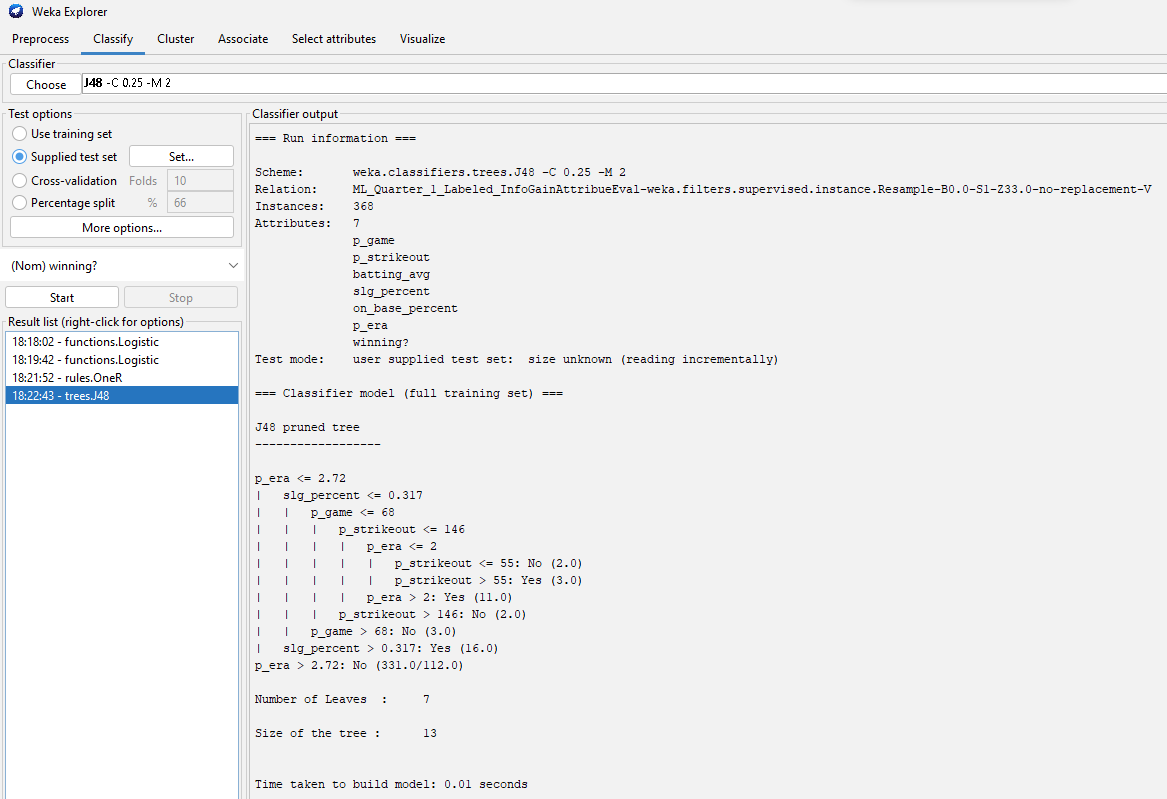
\includegraphics[scale=0.4]{./images/InfoGainAttributeEval/J48-Model.png}
\centering
    \caption{WEKA J48 Model on InfoGainAttributeEval Attributes}
\end{figure}
\newpage
\begin{figure}[h!]
    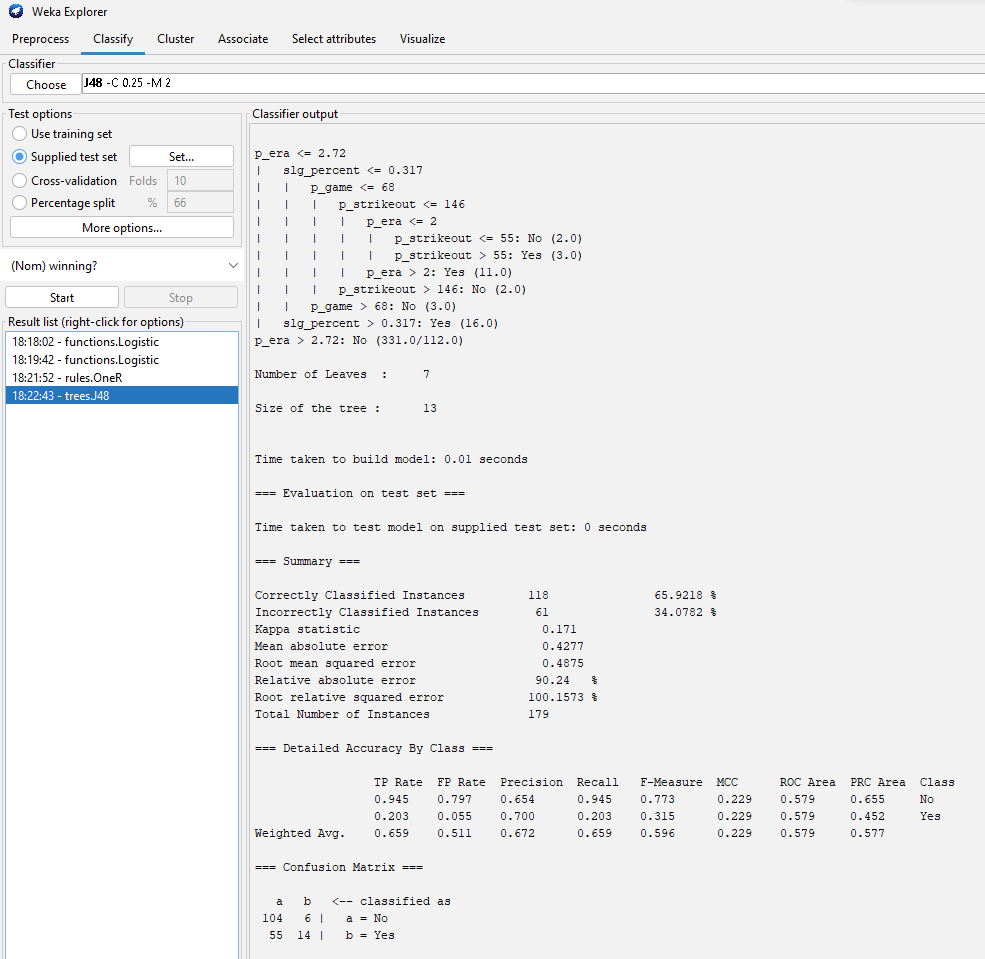
\includegraphics[scale=0.4]{./images/InfoGainAttributeEval/J48-Summary.png}
\centering
    \caption{WEKA J48 Clasifcation Results on InfoGainAttributeEval Attributes}
\end{figure}

\newpage 
\subsubsection{LogisticFunction - InfoGainAttributeEval}
\begin{figure}[h!]
    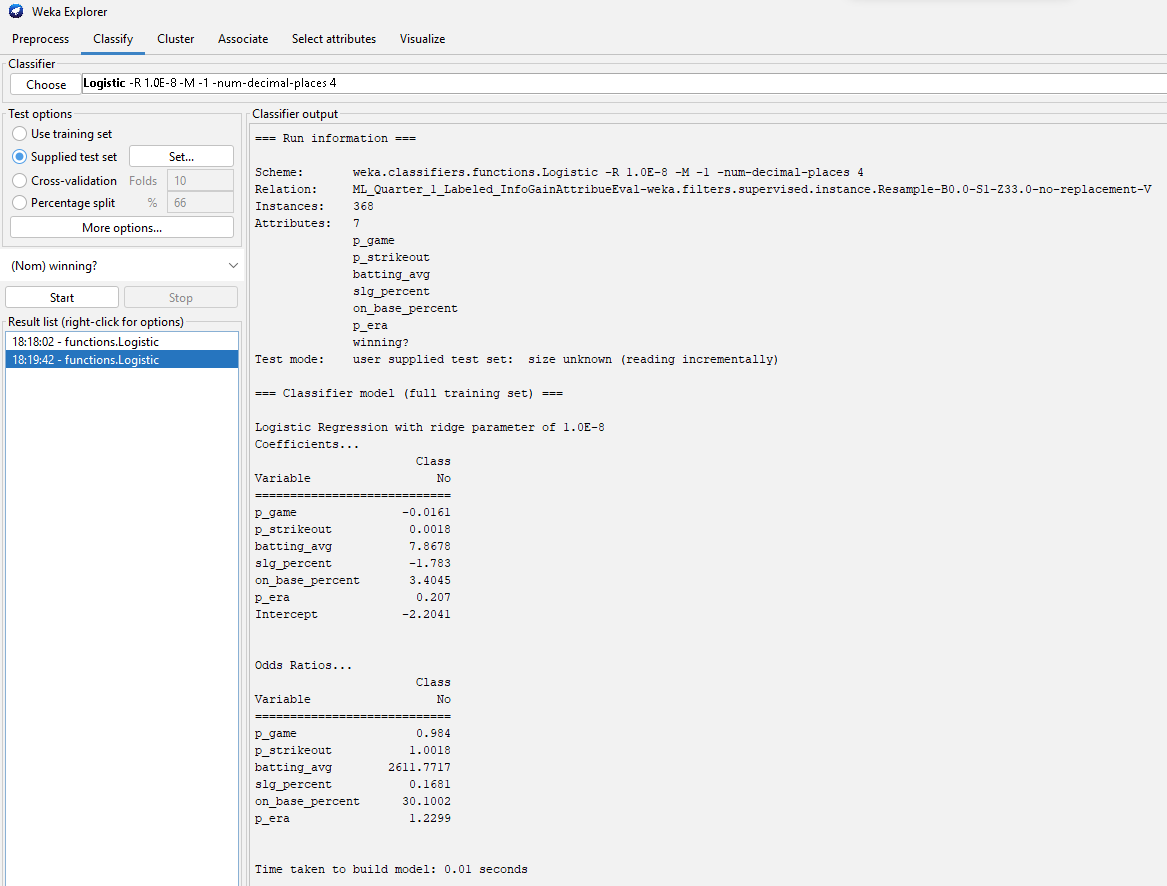
\includegraphics[scale=0.4]{./images/InfoGainAttributeEval/LogisticFunction-Model.png}
\centering
    \caption{WEKA LogisticFunction Model on InfoGainAttributeEval Attributes}
\end{figure}
\newpage
\begin{figure}[h!]
    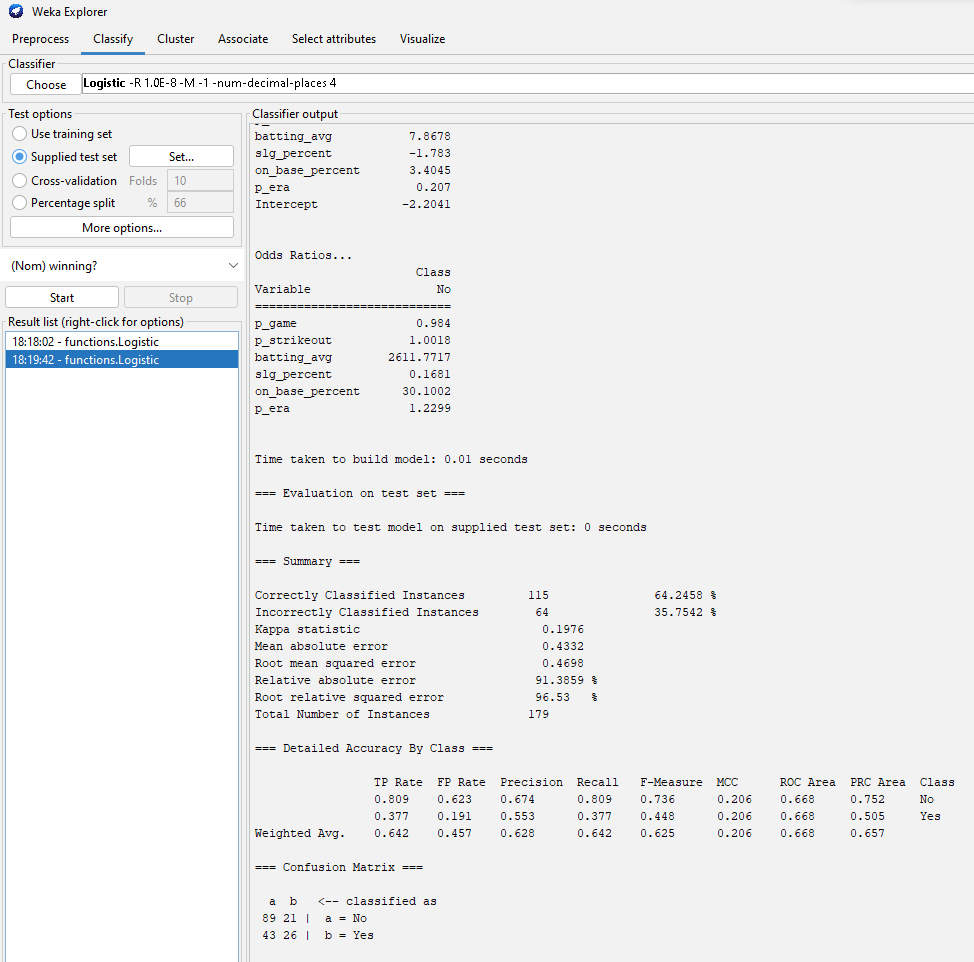
\includegraphics[scale=0.4]{./images/InfoGainAttributeEval/LogisticFunction-Summary.png}
\centering
    \caption{WEKA LogisticFunction Summary Results on InfoGainAttributeEval Attributes}
\end{figure}

\newpage
\subsubsection{Analysis}
$\textbf{J48}$ performed the best with this attribute selection method, with $\textbf{LogisticFunction}$ being a close scond. $\textbf{J48}$ was a lot better at categorizing true positives while $\textbf{LogisticFunction}$ was a lot better at categorizing true negatives. 

\newpage
\subsubsection{NaiveBayes - CorrelationAttributeEval}
\begin{figure}[h!]
    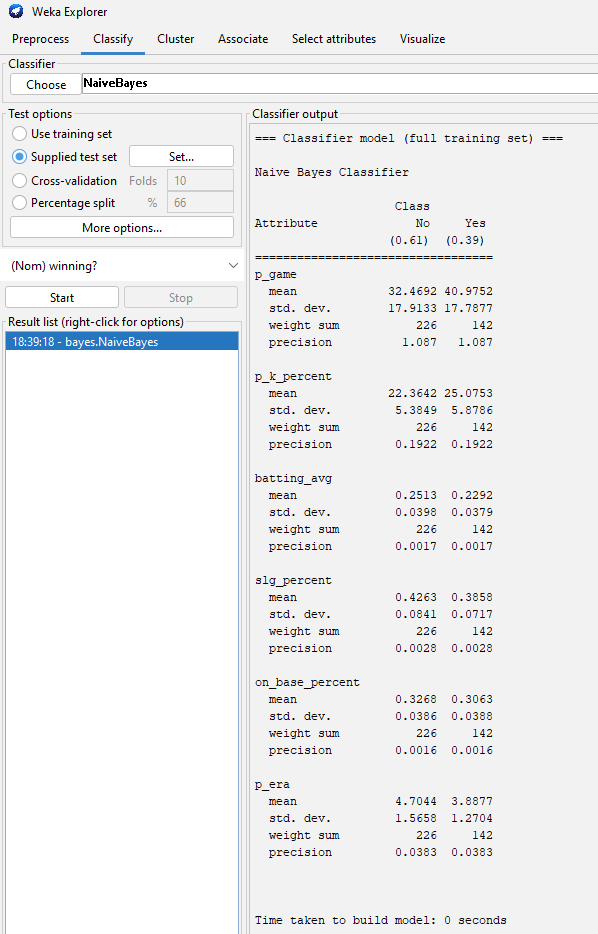
\includegraphics[scale=0.4]{./images/CorrelationAttributeEval/NaiveBayes-Model.png}
\centering
    \caption{WEKA NaiveBayes Model on CorrelationAttributeEval Attributes}
\end{figure}
\newpage
\begin{figure}[h!]
    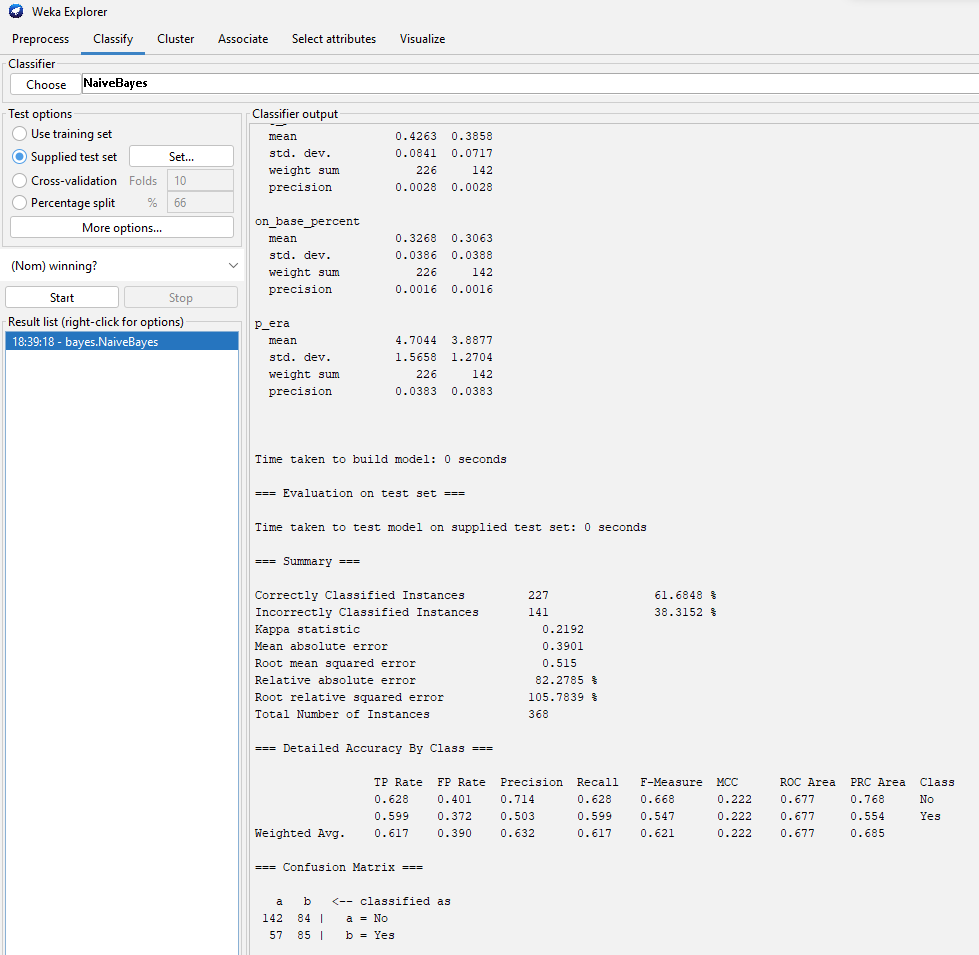
\includegraphics[scale=0.4]{./images/CorrelationAttributeEval/NaiveBayes-Summary.png}
\centering
    \caption{WEKA NaiveBayes Summary Results on CorrelationAttributeEval Attributes}
\end{figure}

\newpage
\subsubsection{OneR - CorrelationAttributeEval}
\begin{figure}[h!]
    \includegraphics[scale=0.4]{./images/CorrelationAttributeEval/OneR-Model.png}
\centering
    \caption{WEKA OneR Model on CorrelationAttributeEval Attributes}
\end{figure}
\newpage
\begin{figure}[h!]
    \includegraphics[scale=0.4]{./images/CorrelationAttributeEval/OneR-Summary.png}
\centering
    \caption{WEKA OneR Summary Results on CorrelationAttributeEval Attributes}
\end{figure}

\newpage
\subsubsection{Analysis}
$\textbf{J48}$ performed the best with this attribute selection method, with $\textbf{LogisticFunction}$ being a close scond. $\textbf{J48}$ was a lot better at categorizing true positives while $\textbf{LogisticFunction}$ was a lot better at categorizing true negatives. This time, $\textbf{LogisticFunction}$ performed a bit worse than normal compared to $\textbf{J48}$. 

\section{Conclusion}
Looking at the data given to us by WEKA, we can see that the best combination of attribute selection and classification method is $\textbf{WrapperSubsetEval}$ and $\textbf{LogisticFunction}$. This method classified with an accuracy of $67.0391\%$. However, with just one more instance misclassified, $\textbf{WraperSubsetEval}$ and $\textbf{J48}$ was a close second. Overall, the best performing models used the $\textbf{WrapperSubsetEval}$ attribute selection method. This is probably due to the fact that it is one of the more complex attribute selection methods, and therefore is more accurate. 

There are many reasons why $\textbf{WrapperSubsetEval}$ and $\textbf{LogisticFunction}$ are better in our case over $\textbf{J48}$. The former had the highest true positive rate $(0.670)$, the lowest false positive rate $(0.423)$, and the highest F-measure $(0.655)$. These three facts combined make $\textbf{WrapperSubsetEval}$ and $\textbf{LogisticFunction}$ the undeniable best attribute selection method and classification method combination. 

Overall, the accuracy of the classifier models was low, with the highest at just over $67\%$. This was surprising because we expected these statistics to be better predictors of performance, but the results make sense given the random nature of baseball and other external factors, like scouting reports and weather that could skew the statistics in some way. 


\section{Discussion}
Throughout the course of this project, we learned a lot about data preprocessing and classification. We learned that well-chosen attributes are essential to having an accurate model, as evidenced by the fact that the attributes that we selected becuase we thought were the most predictive of pitcher performance were actually not the best attributes, and that greatly decreased the accuracy of any classifier algorithm, and even was the worst performing attribute selection method based on the results of the classification methods. This is a classic case of garbage in, garbage out. 

We also learned that sometimes you cannot just compare the accuracy to determine which of two models is better. There needs to be some sort of justification. In our case, the difference between $\textbf{LogisticFunction}$ and $\textbf{J48}$ for the $\textbf{WrapperSubsetEval}$ was almost negligible, but several factors pushed us to determine that $\textbf{LogisticFunction}$ was better. 

Finally, we learned that more is better. It is always better to test out more combinations of classifier models and attribute selection methods. While some are there to provide a baseline estimate, like $\textbf{OneR}$ and $\textbf{NaiveBayes}$, they help provide us with insights if the more complex models go wrong and perform worse than the lightweight ones. Through testing of more combinations, we are more likely to find better performing models. While $\textbf{J48}$ performed the best on most attribute selection methods, it did not perform the best overall, and it would be wrong for us to assume so. If we had not tried out $\textbf{LogisticFunction}$ and $\textbf{WrapperSubsetEval}$, we may not have gotten the same level of performance. 

The work was split evenly between both members during this project, with each person doing half of each step. We collaborated on the best way to handle missing values, and ended up deciding on just deleting rows we found were not needed. We each did three attribute reduction methods, collaborating on the $\textbf{SelfSelected}$ method. We then ran classifier models on the two attribute reduction methods that we each did, and took screenshots of our work. Progress was updated through a git repository, so we always had access to each other\textquotesingle s work. Finally, we collaborated on the writeup and the presentation. 

\section{Sources}
We got our data from \url{https://www.baseballsavant.mlb.com} and used WEKA to preprocess and do classification work. 

Datasets for this project can be found at \url{https://drive.google.com/drive/folders/1sgNZJn71GUput_BZugSGtm8ybw6_6p0P?usp=sharing}. This link includes both the original datasets as well as the modified datasets. 

Research on models was done on both the official WEKA sourceforge site and through \url{https://www.medium.com}. The links to sources used, as well as the original dataset, are in the Bibliography on the next page. 

\newpage
\section{Bibliography}
\url{https://baseballsavant.mlb.com/leaderboard/custom?year=2021&type=pitcher&filter=&sort=2&sortDir=asc&min=100&selections=p_game,p_total_hits,p_home_run,p_strikeout,p_walk,p_k_percent,p_bb_percent,batting_avg,slg_percent,on_base_percent,on_base_plus_slg,p_earned_run,p_win,p_loss,p_era,p_rbi,p_called_strike,p_unearned_run,exit_velocity_avg,launch_angle_avg,sweet_spot_percent,barrel_batted_rate,hard_hit_percent,meatball_percent,pitch_hand,n_fastball_formatted,fastball_avg_speed,n_offspeed_formatted,offspeed_avg_speed,&chart=false&x=p_total_hits&y=p_total_hits&r=no&chartType=beeswarm} \\
\url{https://weka.sourceforge.io/doc.dev/weka/attributeSelection/WrapperSubsetEval.html} \\
\url{https://weka.sourceforge.io/doc.dev/weka/attributeSelection/InfoGainAttributeEval.html} \\
\url{https://weka.sourceforge.io/doc.dev/weka/attributeSelection/GainRatioAttributeEval.html} \\
\url{https://weka.sourceforge.io/doc.dev/weka/attributeSelection/CorrelationAttributeEval.html} \\
\url{https://weka.sourceforge.io/doc.dev/weka/filters/supervised/instance/Resample.html} \\
\url{https://medium.com/@nilimakhanna1/j48-classification-c4-5-algorithm-in-a-nutshell-24c50d20658e} \\
\url{https://medium.com/swlh/lets-talk-logistic-regression-4b2072ad7b4e} \\
\url{https://medium.com/x8-the-ai-community/a-simple-introduction-to-naive-bayes-23538a0395a} \\
\url{https://medium.com/squad-engineering/one-class-classification-for-images-with-deep-features-69182fb4c9c5}

\end{document}
